\documentclass[a4paper,11pt,fleqn,twoside,openright]{memoir} 	% Openright aabner kapitler paa hoejresider (openany begge)

%%%% PACKAGES %%%%

% ¤¤ Oversaettelse og tegnsaetning ¤¤ %
\usepackage[utf8]{inputenc}					% Input-indkodning af tegnsaet (UTF8)
\usepackage[english]{babel}					% Dokumentets sprog
\usepackage[T1]{fontenc}					% Output-indkodning af tegnsaet (T1)
\usepackage{ragged2e,anyfontsize}			% Justering af elementer
\usepackage{fixltx2e}						% Retter forskellige fejl i LaTeX-kernen
																			
% ¤¤ Figurer og tabeller (floats) ¤¤ %
\usepackage{graphicx} 						% Haandtering af eksterne billeder (JPG, PNG, PDF)
\usepackage{multirow}                		% Fletning af raekker og kolonner (\multicolumn og \multirow)
\usepackage{colortbl} 						% Farver i tabeller (fx \columncolor, \rowcolor og \cellcolor)
\usepackage[dvipsnames]{xcolor}				% Definer farver med \definecolor. Se mere: http://en.wikibooks.org/wiki/LaTeX/Colors
\usepackage{flafter}						% Soerger for at floats ikke optraeder i teksten foer deres reference
\let\newfloat\relax 						% Justering mellem float-pakken og memoir
\usepackage{float}							% Muliggoer eksakt placering af floats, f.eks. \begin{figure}[H]
%\usepackage{eso-pic}						% Tilfoej billedekommandoer paa hver side
%\usepackage{wrapfig}						% Indsaettelse af figurer omsvoebt af tekst. \begin{wrapfigure}{Placering}{Stoerrelse}
%\usepackage{multicol}         	        	% Muliggoer tekst i spalter
%\usepackage{rotating}						% Rotation af tekst med \begin{sideways}...\end{sideways}
\usepackage{array}


% ¤¤ Matematik mm. ¤¤
\usepackage{amsmath,amssymb,stmaryrd} 		% Avancerede matematik-udvidelser
\usepackage{mathtools}						% Andre matematik- og tegnudvidelser
\usepackage{textcomp}                 		% Symbol-udvidelser (f.eks. promille-tegn med \textperthousand )
\usepackage{siunitx}						% Flot og konsistent praesentation af tal og enheder med \si{enhed} og \SI{tal}{enhed}
\sisetup{output-decimal-marker = {,}}		% Opsaetning af \SI (DE for komma som decimalseparator) 
\usepackage[version=3]{mhchem} 				% Kemi-pakke til flot og let notation af formler, f.eks. \ce{Fe2O3}
%\usepackage{rsphrase}						% Kemi-pakke til RS-saetninger, f.eks. \rsphrase{R1}

% ¤¤ Referencer og kilder ¤¤ %
\usepackage[danish]{varioref}				% Muliggoer bl.a. krydshenvisninger med sidetal (\vref)
\usepackage{natbib}							% Udvidelse med naturvidenskabelige citationsmodeller
%\usepackage{xr}							% Referencer til eksternt dokument med \externaldocument{<NAVN>}
%\usepackage{glossaries}					% Terminologi- eller symbolliste (se mere i Daleifs Latex-bog)

% ¤¤ Misc. ¤¤ %
\usepackage{listings}						% Placer kildekode i dokumentet med \begin{lstlisting}...\end{lstlisting}
\usepackage{lipsum}							% Dummy text \lipsum[..]
\usepackage[shortlabels]{enumitem}			% Muliggoer enkelt konfiguration af lister
\usepackage{pdfpages}						% Goer det muligt at inkludere pdf-dokumenter med kommandoen \includepdf[pages={x-y}]{fil.pdf}	
\pdfoptionpdfminorversion=6					% Muliggoer inkludering af pdf dokumenter, af version 1.6 og hoejere
\pretolerance=2500 							% Justering af afstand mellem ord (hoejt tal, mindre orddeling og mere luft mellem ord)

% Kommentarer og rettelser med \fxnote. Med 'final' i stedet for 'draft' udloeser hver note en error i den faerdige rapport.
\usepackage[footnote,draft,danish,silent,nomargin]{fixme}		

\usepackage{todonotes}

\usepackage{lastpage}

%%%% CUSTOM SETTINGS %%%%

% ¤¤ Marginer ¤¤ %
\setlrmarginsandblock{3.5cm}{2.5cm}{*}		% \setlrmarginsandblock{Indbinding}{Kant}{Ratio}
\setulmarginsandblock{2.5cm}{3.0cm}{*}		% \setulmarginsandblock{Top}{Bund}{Ratio}
\checkandfixthelayout 						% Oversaetter vaerdier til brug for andre pakker

%	¤¤ Afsnitsformatering ¤¤ %
\setlength{\parindent}{0mm}           		% Stoerrelse af indryk
\setlength{\parskip}{3mm}          			% Afstand mellem afsnit ved brug af double Enter
\linespread{1,1}							% Linie afstand

% ¤¤ Litteraturlisten ¤¤ %
\bibpunct[,]{[}{]}{;}{a}{,}{,} 				% Definerer de 6 parametre ved Harvard henvisning (bl.a. parantestype og seperatortegn)
\bibliographystyle{bibtex/harvard}			% Udseende af litteraturlisten.

% ¤¤ Indholdsfortegnelse ¤¤ %
\setsecnumdepth{subsection}		 			% Dybden af nummerede overkrifter (part/chapter/section/subsection)
\maxsecnumdepth{subsection}					% Dokumentklassens graense for nummereringsdybde
\settocdepth{subsection} 					% Dybden af indholdsfortegnelsen

% ¤¤ Lister ¤¤ %
\setlist{
  topsep=0pt,								% Vertikal afstand mellem tekst og listen
  itemsep=-1ex,								% Vertikal afstand mellem items
} 

% ¤¤ Visuelle referencer ¤¤ %
\usepackage[colorlinks]{hyperref}			% Danner klikbare referencer (hyperlinks) i dokumentet.
\hypersetup{colorlinks = true,				% Opsaetning af farvede hyperlinks (interne links, citeringer og URL)
    linkcolor = black,
    citecolor = black,
    urlcolor = black
}

% ¤¤ Opsaetning af figur- og tabeltekst ¤¤ %
\captionnamefont{\small\bfseries\itshape}	% Opsaetning af tekstdelen ('Figur' eller 'Tabel')
\captiontitlefont{\small}					% Opsaetning af nummerering
\captiondelim{. }							% Seperator mellem nummerering og figurtekst
\hangcaption								% Venstrejusterer flere-liniers figurtekst under hinanden
\captionwidth{\linewidth}					% Bredden af figurteksten
\setlength{\belowcaptionskip}{0pt}			% Afstand under figurteksten
		
% ¤¤ Opsaetning af listings ¤¤ %
\definecolor{commentGreen}{RGB}{34,139,24}
\definecolor{stringPurple}{RGB}{208,76,239}

\lstset{language=Matlab,					% Sprog
	basicstyle=\ttfamily\scriptsize,		% Opsaetning af teksten
	keywords={for,if,while,else,elseif,		% Noegleord at fremhaeve
			  end,break,return,case,
			  switch,function},
	keywordstyle=\color{blue},				% Opsaetning af noegleord
	commentstyle=\color{commentGreen},		% Opsaetning af kommentarer
	stringstyle=\color{stringPurple},		% Opsaetning af strenge
	showstringspaces=false,					% Mellemrum i strenge enten vist eller blanke
	numbers=left, numberstyle=\tiny,		% Linjenumre
	extendedchars=true, 					% Tillader specielle karakterer
	columns=flexible,						% Kolonnejustering
	breaklines, breakatwhitespace=true,		% Bryd lange linjer
}

% ¤¤ Navngivning ¤¤ %
%\addto\captionsdanish{
%	\renewcommand\appendixname{Appendiks}
%	\renewcommand\contentsname{Indholdsfortegnelse}	
%	\renewcommand\appendixpagename{Appendiks}
%	\renewcommand\appendixtocname{Appendiks}
%	\renewcommand\cftchaptername{\chaptername~}				% Skriver "Kapitel" foran kapitlerne i indholdsfortegnelsen
%	\renewcommand\cftappendixname{\appendixname~}			% Skriver "Appendiks" foran appendiks i indholdsfortegnelsen
%	}

% ¤¤ Kapiteludssende ¤¤ %
\definecolor{numbercolor}{gray}{0.7}		% Definerer en farve til brug til kapiteludseende
\newif\ifchapternonum

\makechapterstyle{jenor}{					% Definerer kapiteludseende frem til ...
  \renewcommand\beforechapskip{0pt}
  \renewcommand\printchaptername{}
  \renewcommand\printchapternum{}
  \renewcommand\printchapternonum{\chapternonumtrue}
  \renewcommand\chaptitlefont{\fontfamily{pbk}\fontseries{db}\fontshape{n}\fontsize{25}{35}\selectfont\raggedleft}
  \renewcommand\chapnumfont{\fontfamily{pbk}\fontseries{m}\fontshape{n}\fontsize{1in}{0in}\selectfont\color{numbercolor}}
  \renewcommand\printchaptertitle[1]{%
    \noindent
    \ifchapternonum
    \begin{tabularx}{\textwidth}{X}
    {\let\\\newline\chaptitlefont ##1\par} 
    \end{tabularx}
    \par\vskip-2.5mm\hrule
    \else
    \begin{tabularx}{\textwidth}{Xl}
    {\parbox[b]{\linewidth}{\chaptitlefont ##1}} & \raisebox{-15pt}{\chapnumfont \thechapter}
    \end{tabularx}
    \par\vskip2mm\hrule
    \fi
  }
}											% ... her

\chapterstyle{jenor}						% Valg af kapiteludseende - Google 'memoir chapter styles' for alternativer

% ¤¤ Sidehoved ¤¤ %

\makepagestyle{Uni}							% Definerer sidehoved og sidefod udseende frem til ...
\makepsmarks{Uni}{%
	\createmark{chapter}{left}{shownumber}{}{. \ }
	\createmark{section}{right}{shownumber}{}{. \ }
	\createplainmark{toc}{both}{\contentsname}
	\createplainmark{lof}{both}{\listfigurename}
	\createplainmark{lot}{both}{\listtablename}
	\createplainmark{bib}{both}{\bibname}
	\createplainmark{index}{both}{\indexname}
	\createplainmark{glossary}{both}{\glossaryname}
}
\nouppercaseheads											% Ingen Caps oenskes

\makeevenhead{Uni}{Gruppe B131}{}{\leftmark}				% Definerer lige siders sidehoved (\makeevenhead{Navn}{Venstre}{Center}{Hoejre})
\makeoddhead{Uni}{\rightmark}{}{Dit Universitet}			% Definerer ulige siders sidehoved (\makeoddhead{Navn}{Venstre}{Center}{Hoejre})
\makeevenfoot{Uni}{\thepage}{}{}							% Definerer lige siders sidefod (\makeevenfoot{Navn}{Venstre}{Center}{Hoejre})
\makeoddfoot{Uni}{}{}{\thepage}								% Definerer ulige siders sidefod (\makeoddfoot{Navn}{Venstre}{Center}{Hoejre})
\makeheadrule{Uni}{\textwidth}{0.5pt}						% Tilfoejer en streg under sidehovedets indhold
\makefootrule{Uni}{\textwidth}{0.5pt}{1mm}					% Tilfoejer en streg under sidefodens indhold

\copypagestyle{Unichap}{Uni}								% Sidehoved for kapitelsider defineres som standardsider, men med blank sidehoved
\makeoddhead{Unichap}{}{}{}
\makeevenhead{Unichap}{}{}{}
\makeheadrule{Unichap}{\textwidth}{0pt}
\aliaspagestyle{chapter}{Unichap}							% Den ny style vaelges til at gaelde for chapters
															% ... her
															
\pagestyle{Uni}												% Valg af sidehoved og sidefod (benyt "plain" for ingen sidehoved/fod)


%%%% CUSTOM COMMANDS %%%%

% ¤¤ Billede hack ¤¤ %										% Indsaet figurer nemt med \figur{Stoerrelse}{Fil}{Figurtekst}{Label}
\newcommand{\figur}[4]{
		\begin{figure}[H] \centering
			\includegraphics[width=#1\textwidth]{billeder/#2}
			\caption{#3}\label{#4}
		\end{figure} 
}

% ¤¤ Specielle tegn ¤¤ %
\newcommand{\decC}{^{\circ}\text{C}}
\newcommand{\dec}{^{\circ}}
\newcommand{\m}{\cdot}


%%%% ORDDELING %%%%

\hyphenation{}											% Preamble indlaeses
\raggedbottom													% Soerger for at LaTeX ikke "straekker" teksten

%\includeonly{file1,file2}										% Inkluder kun specifikke filer (kommasepareret liste)

\begin{document}												% Starter dokumentet - obligatorisk


\frontmatter													% Forindhold - nummereres med romertal

\thispagestyle{empty}
\begin{flushright}
\vspace{3cm}

\phantom{hul}

\phantom{hul}

\phantom{hul}

\textsl{\Huge Energirenovering} \\ \vspace{1cm}

\rule{13cm}{3mm} \\ \vspace{1.5cm}
\vspace{1cm}

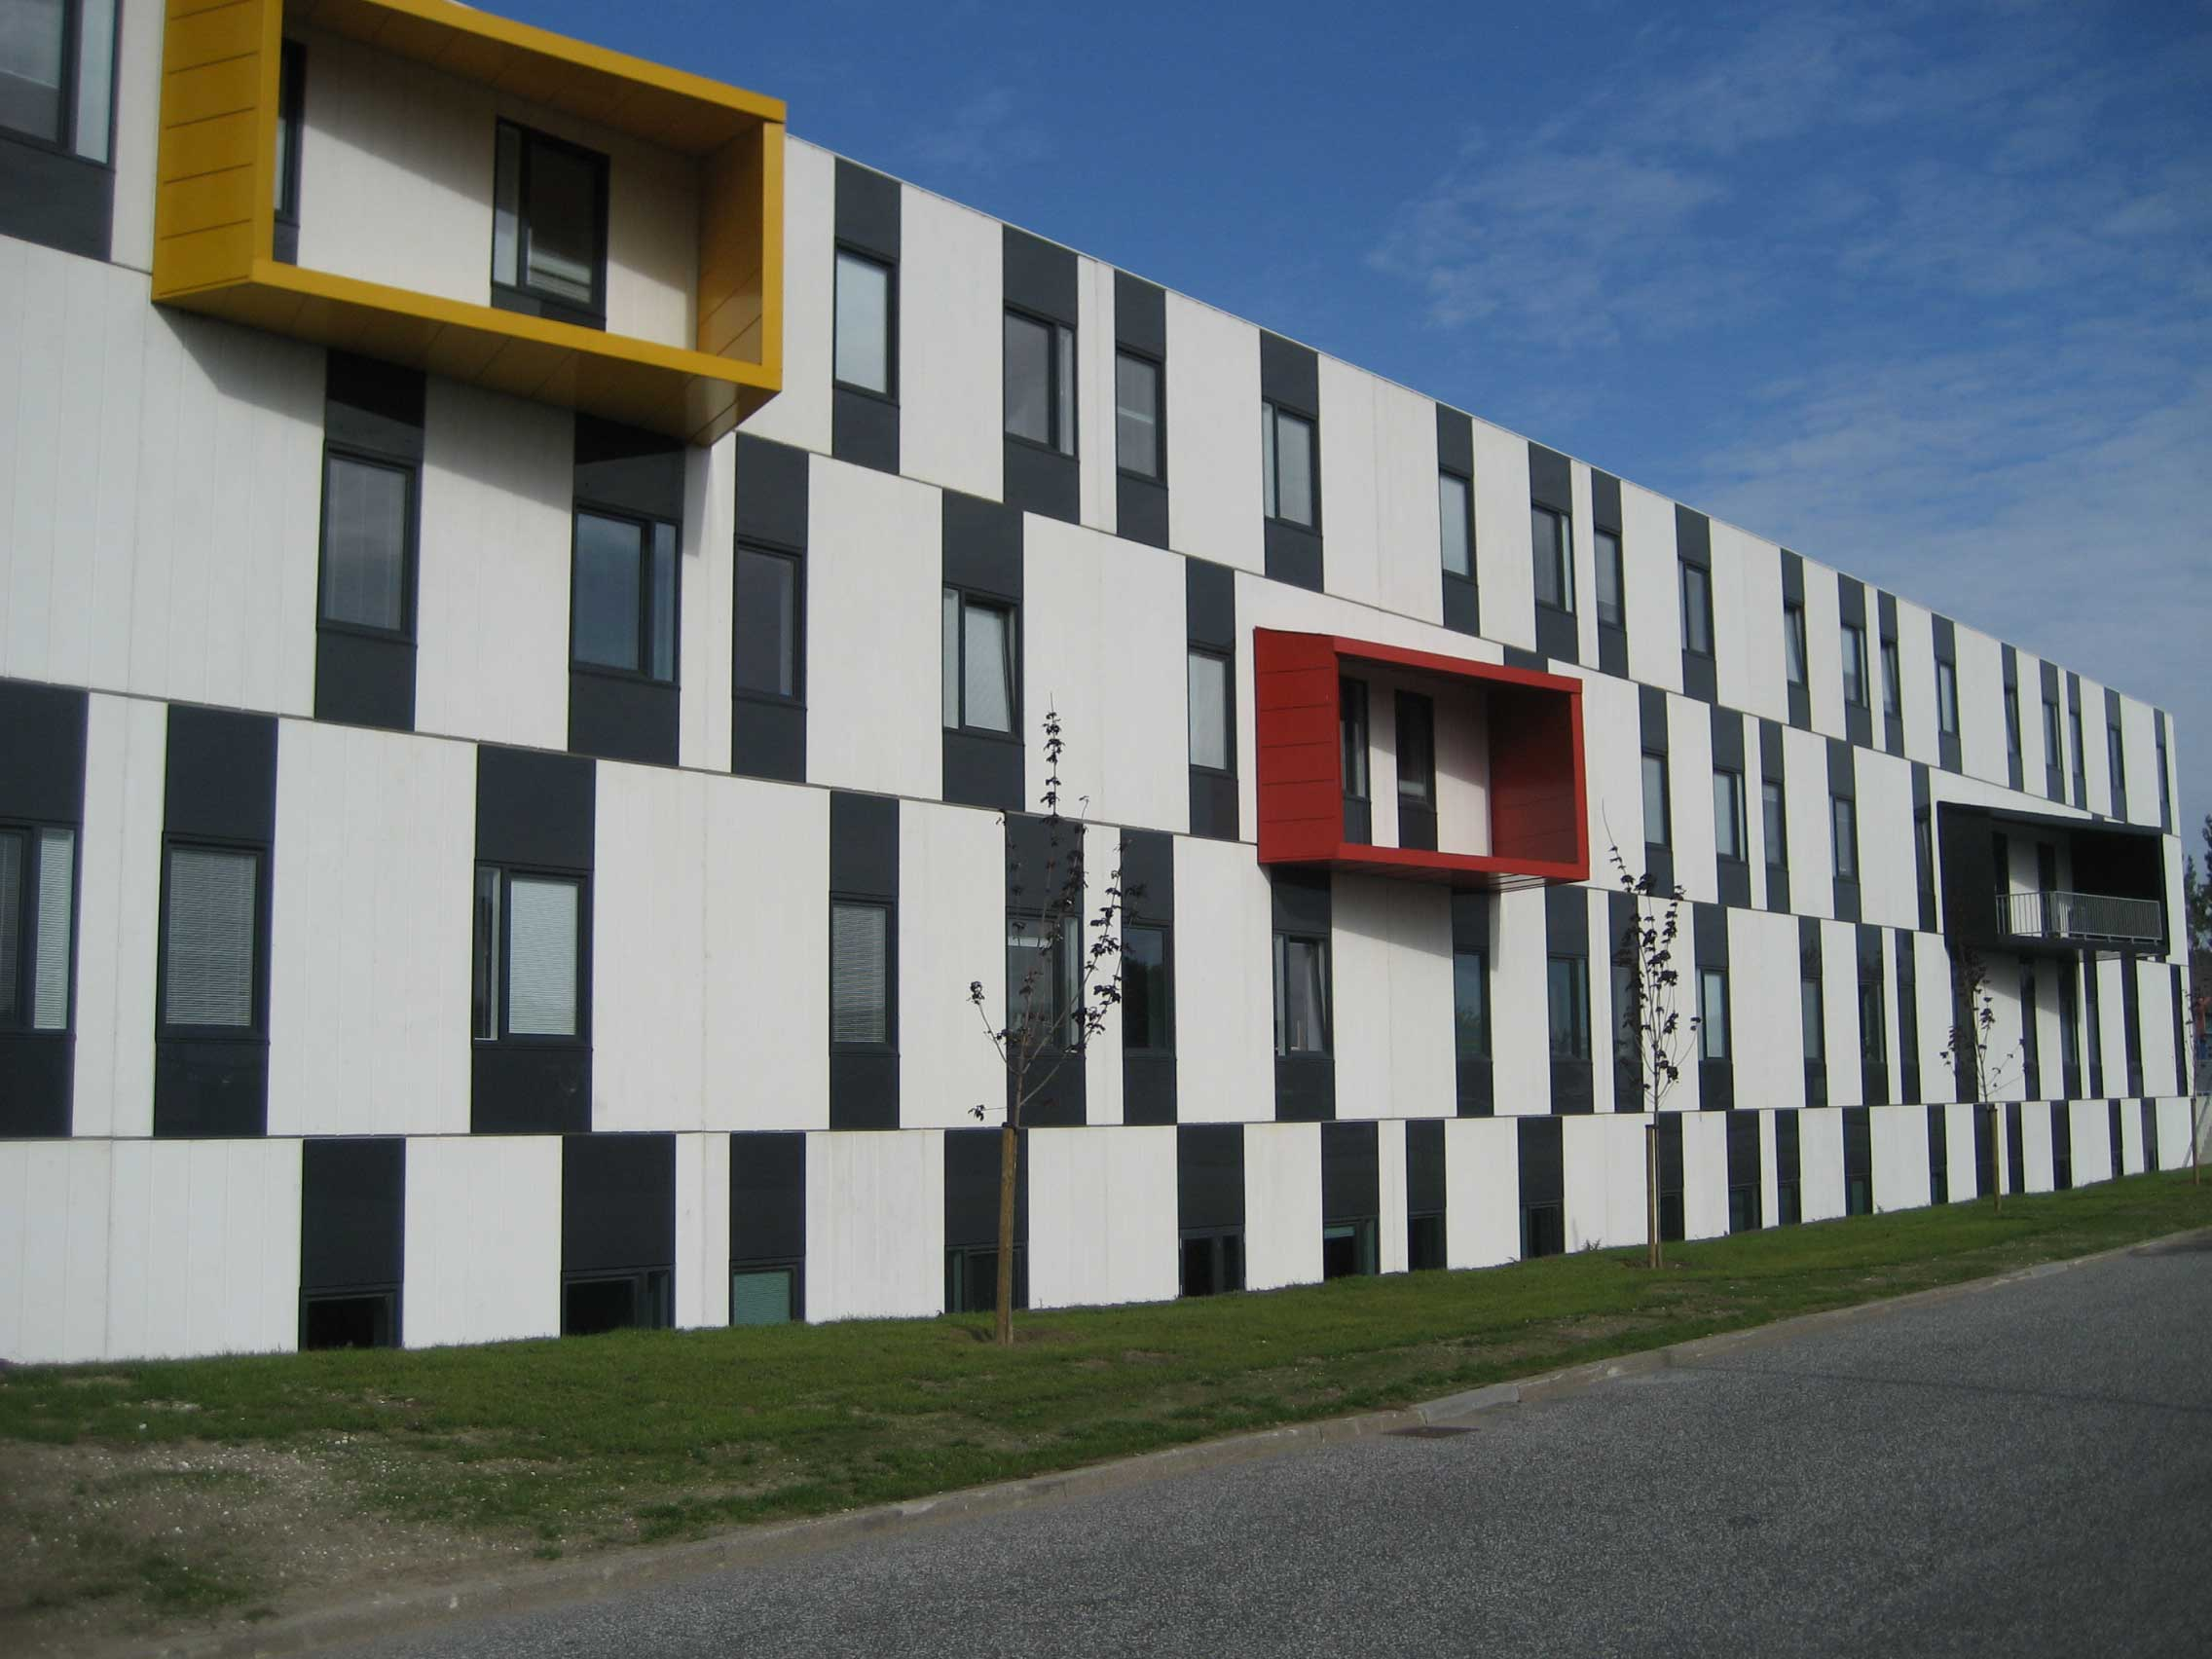
\includegraphics[width=0.9\textwidth]{billeder/forside.jpg}

\vspace{2cm} 
\textsc{\Large P4 Project \\
Group sw408f16 \\
Software\\
Aalborg Universitet\\
Den 26. maj 2016\\}
\end{flushright}

\cleardoublepage												% Indsaetter tom side, saa naeste kapitel starter paa hoejre side (hvis noedvendigt)
% Dette er LaTeX-versionen af titelbladet for TNB studenterrapporter
% Filen kræver:
% Universitetets logo:  AAU-logo-stud-UK eller AAU-logo-stud-DK
% Synopsis: En fil ved navn synopsis.tex

% Udarbejdet af: Jesper Nørgaard (jesper@noergaard.eu) 10. april 2012

\phantomsection
\pdfbookmark[0]{Titelblad}{titelblad}
\thispagestyle{empty}

\begin{minipage}[t]{0.48\textwidth}
\vspace*{-25pt}			%\vspace*{-9pt}

\includegraphics[height=4cm]{billeder/AAU-logo-stud-DK-RGB}
\end{minipage}
\hfill
\begin{minipage}[t]{0.48\textwidth}
{\small 
\textbf{Første Studieår v/ Det Teknisk-}\\
\textbf{Naturvidenskabelige Fakultet}  \\
Byggeri og Anlæg \\
Strandvejen 12-14 \\
9000 Aalborg \\
http://www.tnb.aau.dk}
\end{minipage}

\vspace*{1cm}

\begin{minipage}[t]{0.48\textwidth}
\textbf{Titel:} \\[5pt]\bigskip\hspace{2ex}
Energirenovering

\textbf{Projekt:} \\[5pt]\bigskip\hspace{2ex}
P1-projekt

\textbf{Projektperiode:} \\[5pt]\bigskip\hspace{2ex}
September 2014 - December 2014

\textbf{Projektgruppe:} \\[5pt]\bigskip\hspace{2ex}
B131	

\textbf{Deltagere:} \\[5pt]\hspace*{2ex}
Adam  G. Hansen \\\hspace*{2ex}
Berit Jørgensen \\\hspace*{2ex}
Christoffer Haning \\\hspace*{2ex}
Dorthe Møller \\\hspace*{2ex}
Ejnar V. Jensen \\\hspace*{2ex}
Freja Poulsen \\\bigskip\hspace{2ex}
Gerhard Pedersen

\textbf{Vejledere:} \\[5pt]\hspace*{2ex}
Carsten Henningsen \\\bigskip\hspace{2ex}
Lotte Dalgaard

\vspace*{1cm}

\textbf{Oplagstal: 10} \\
\textbf{Sidetal: 80} \\
\textbf{Appendiks: 3} \\ 
\textbf{Afsluttet 18-12-2014}

\end{minipage}
\hfill
\begin{minipage}[t]{0.483\textwidth}
Synopsis: \\[5pt]
\fbox{\parbox{7cm}{\bigskipSynopsis

\bigskip}}
\end{minipage}

\vfill

{\footnotesize\itshape Rapportens indhold er frit tilgængeligt, men offentliggørelse (med kildeangivelse) må kun ske efter aftale med forfatterne.}

% Rapportens indhold er frit tilgængeligt, men offentliggørelse (med kildeangivelse) må kun ske efter aftale med forfatterne.
% The content of the report is freely available, but publication (with source reference) may only take place in agreement with the authors.

\cleardoublepage
\chapter*{Forord}

Denne rapport er udarbejdet af en gruppe studerende på 1. semester på Byggeri og Anlægs-uddannelsen ved Aalborg Universitet. \textit{Byggeboom i Aalborg} er det overordnede tema for projektet.

Fra projektkataloget er der valgt projektet \textit{Energirenovering}, som lægger op til at belyse andre sider af et byggeboom. Projektet omfatter en kontekstuel vinkel og en teknisk vinkel. Den tekniske del belyser faglighederne energi og indeklima samt konstruktion. Den konstekstuelle del af rapporten behandler ...

Forudsætningerne for at læse rapporten er et vist kendskab til ... \\
Der rettes stor tak til vejlederne ... for inspirerende vejledning og konstruktiv kritik. Endvidere rettes en stor tak til ...

\textbf{Læsevejledning}

Der vil igennem rapporten fremtræde kildehenvisninger, og disse vil være samlet i en kildeliste bagerst i rapporten. Der er i rapporten anvendt kildehenvisning efter Harvardmetoden, så i teksten refereres en kilde med [Efternavn, År]. Denne henvisning fører til kildelisten, hvor bøger er angivet med forfatter, titel, udgave og forlag, mens Internetsider er angivet med forfatter, titel og dato. Figurer og tabeller er nummereret i henhold til kapitel, dvs. den første figur i kapitel 7 har nummer 7.1, den anden, nummer 7.2 osv. Forklarende tekst til figurer og tabeller findes under de givne figurer og tabeller.

\phantom{Luft}

\phantom{Luft}

\begin{table}[H]
	\centering
		\begin{tabular}{c c c}
			\underline{\phantom{mmmmmmmmmmmmmm}} & \underline{\phantom{mmmmmmmmmmmmmm}} & \underline{\phantom{mmmmmmmmmmmmmm}} \\
			Adam  G. Hansen			& Berit Jørgensen 		& Christoffer Haning 			\\
			&&\\
			&&\\
			\underline{\phantom{mmmmmmmmmmmmmm}} & \underline{\phantom{mmmmmmmmmmmmmm}} & \underline{\phantom{mmmmmmmmmmmmmm}} \\
			Dorthe Møller			& Ejnar V. Jensen 		& Freja Poulsen 				\\
			&&\\
			&&\\
		 							& \underline{\phantom{mmmmmmmmmmmmmm}} 	&			\\														
									& Gerhard Pedersen 							& 												
		\end{tabular}
\end{table}
\cleardoublepage

%%%% Indholdsfortegnelse (TOC) %%%%

\phantomsection													% Kunstigt afsnit, som hyperlinks kan 'holde fast i'
\pdfbookmark[0]{Indholdsfortegnelse}{indhold}					% Tildeler en klikbar bookmark til den endelige PDF
\tableofcontents*												% Indholdsfortegnelsen (kaldet ToC) 

%\addtocontents{toc}{\protect\newpage}							% Fremtvinger sideskift i ToC hvis noedvendig (der hvor koden placeres)


\mainmatter														% Hovedindhold - nummereres fra side 1

%%%% Rapportindhold %%%% 										% Rapportindholdet boer IKKE indeholde broedtekst - KUN includede filer!

%% Indledende %%												% Opdel evt. i passende afsnit for overblikkets skyld

\chapter{Introduction}

In Danish high schools all kinds of different languages are available for the students, and the programming languages has found their place as well. For beginners, the syntactic rules, type systems and the nature of the language can be hard to comprehend at first, which is why this report will focus on constructing a language for the high school students. The interest for computer games in the 21st century is bigger than ever \citep{Wankel}, and computer games is a fun and educating approach to learning programming languages. Robocode is a game where the player has to code their own robot, giving every player the opportunity to battle each other’s robots, making it a competition of coding the ‘best’ robot. This is mainly coded in Java, which is an object oriented programming language, and this nature of the language can be hard to understand without having programming experience. There is no popular domain-specific language for Robocode, and therefore the high school students, who is not experienced programmers, may not be likely to code a working robot. This is due to the fact that it requires one to know an object oriented language in advance. 

This is a problem, since Robocode could potentially be a great way of introducing these students for programming languages. If there was a domain-specific language, with more intuitive type systems and good writability, students could easily be introduced for a programming language, and afterwards expand their knowledge gradually on a general purpose programming language. In this report, Robocode will be studied, and the final product should be a domain-specific language for Robocode, compiled to Java.
	
Based on the above mentioned introduction, the project will try to answer the following problem statement:

\textbf{How can a domain-specific language for Robocode simplify the creation of a robot for high school students, with little or no experience to programming?} 
\begin{itemize}
	\item How can the Java type system be simplified?
	\item Which constructs are necessary for programming standard robots in Robocode?
	\item How can an easy to use interface be made for the users?
\end{itemize}
\chapter{Analysis}
\label{chap:Analysis}
The analysis chapter is of purpose to create a basis for the further work with developing a programming language to make the use of Robocode easier for new programmers. This chapter contains a description of Robocode and cover the basics of how to use it. 

Further in the analysis the choice of a parser generator for the project will be discussed. The work of the analysis has the purpose of leading to the next chapter, \ref{chap:LanguageDesign}.

\section{Robocode}
\label{sec:Robocode}
Robocode is an Open Source game project on SourceForge originally started by Mathew A. Nelson in late 2000, who was inspired by RobotBattle from the 1990s. Contributors for the Open Source lead to two new projects, RobocodeNG and Robocode 2006, by Flemming N. Larsen. These two new versions had bug fixes, and new features by the community of Robocode, and in 2006 Flemming merged one of the projects, the Robocode 2006, into an official version 1.1.
The Robocode client was introduced in May 2007, which can be used to create the robots for the game. These robots are usually coded in Java, but in the recent years, C\# and Scala are popular as well. \citep{robocode}

In schools and universities, Robocode is introduced for education and research purposes, as it is intended to be fun and easy to understand the core principles: One robot each, with abilities to drive forward, backwards, turn to the sides, and shoot a gun. These core principles can be vastly expanded to more complicated demands, as the robots universe is bigger than it looks at a first glance. \citep{RoboReadMe}

The way this game works, is by writing code in one of their supported programming languages and then setting it into battle with other people’s robots. There are some sample robots, when the game is downloaded, in order to give the users/players a chance to see how it’s supposed to be written and from there, it’s up to the single individual to make the “best” robot. \citep{MyFirstRobot}

There are held tournaments around the world, where people from around the globe compete. It varies in size, some tournaments are only country based, while others are worldwide, some have leagues and the options are more or less limitless. \citep{rc}

As mentioned before, the Robocode is usually coded in Java, which leads to this report only examining Java samples. This is to prevent any misleading keywords or misinterpretations. The Robocode client comes with a text editor, and the sample robots. In this chapter, some of these sample robots will be examined, and the general setup and main events or methods will be presented.

When creating a new robot in the Robocode text editor, the following methods and events are present:

\begin{lstlisting}[caption={Eksampel of the main loop in Robocode} label=run, xleftmargin=.2\textwidth]
public void run() {
	while(true) {
		//Robots behaviour
	}
}
\end{lstlisting}

This method is the loop for the robot, this loop will determine what the robot does constantly, unless interrupted by an event, which the user can define. The robot behaviour is what the user will code as the AI, along with the robot behaviour in the following code snippets.

\begin{lstlisting}[caption={Eksampel of the onScannedRobot event from Robocode} label=osr, xleftmargin=.2\textwidth]
public void onScannedRobot(ScannedRobotEvent e) {
	//Robots behaviour
}
\end{lstlisting}

The robot’s radar will spot enemies when they get within the vision of the radar, which will raise the onScannedRobot event. This event is used to determine how the robot reacts to spotting an enemy, where the ScannedRobotEvent e is the source for information about the enemy robot spotted.

\begin{lstlisting}[caption={Eksampel of the onHitByBullet event from Robocode} label=ohbb, xleftmargin=.2\textwidth]
public void onHitByBullet(HitByBulletEvent e) {
	//Robots behaviour
}
\end{lstlisting}

When the robot gets hit by another robot’s bullet, the event onHitByBullet will be raised. The robot can then be programmed to act a specific way, change behaviour or carry out a task when the event is raised.

\begin{lstlisting}[caption={Eksampel of the onHitWall event from Robocode} label=ohw, xleftmargin=.2\textwidth]
public void onHitWall(HitWallEvent e) {
	//Robots behaviour
}
\end{lstlisting}

When the robot drives into the wall, the event onHitWall will be raised, and the robot can be programmed to do a specific task when this occurs. 

The above mentioned is only a few of the events that can occur in Robocode. In the while loop, events and functions the user can use many build-in methods from the robot class, which is moving and controlling the robot, controlling the radar and the gun and getting information about the battlefield, the user's robot, other robots and many other things. 


In this section the robocode concept will be described. It will include the different functions the system contains.
  
\subsection{Robot}
The robot is the core of the game. The robot can be coded to act differently in various of encounters. There are some events in Robocode that the users can use to program their strategies. One of the events could be onHitWall which basically tells the user that if the robot hits the wall, then the robot will execute the code matches the event that occurred. The robots also have a gun. The gun is used to damage antagonist robots, in the arena. The robot has a gun, and the possibility to choose different types of bullets. For example, one play could use small and fast bullets, they won’t necessarily hurt very much, but it allows the player to shoot more frequent, compared to larger slower bullets. 

The robot also has a radar. The radar allows the robot to scan for other robots scan and walls. This could once again affect the strategies of the robots.

\subsection{Battlefield}
The battlefield is the arena where the robots will fight each other. It’s also the visible field on screen when the game is running. When coding, the battlefield can be used for different reasons, for example, to get the number of enemies that are alive. A robot might be programmed to act differently if there are less than three robots left. All this depends on the way the player decided to program his robot. Some of the other examples that the battlefield can be queried or could be the field size, time or the current round number. 

\subsection{Energy}
Robots have energy, which is the spendable resource when shooting bullets, it is the ‘health’ of a robot, since being hit by a wall or another robots bullet causes a robot to lose energy. But if one robot hits another one, it regains energy. All robots start at 100 energy at the start of a fight, but can exceed this amount, by hitting other robots to regain energy, without losing it. The amount of energy gained when hitting a robot is (3 * bulletpower), which is three times the power you spend shooting it. By being hit by a bullet, the robot lose (4 * bulletpower), and hitting a wall with an AdvancedRobot extended robot will cause the robot to lose energy as well.

If a robot shoots a bullet which uses the last energy that particular robot has, it will be disabled. A disabled robot will not be able to move or shoot. The last shot that robot took, has a chance to restore the robot, if it hits an enemy and thereby regaining energy.
   
Energy for the robots are both the health and the spendable resource for attacking, which makes every decision of manoeuvring and shooting count.

\subsection{Scoring}
Winning in robocode is not about being the sole survivor, not even in the RoboRumble gamemode, which is the “every man for himself” type of gamemode. It is all about scoring, and there are different methods for scoring points. The various types of scoring are as following:
\begin{itemize}
\item Survival score, every time a robot dies, all remaining robots get 50 points.
\item Last survivor bonus, the last robot alive scores 10 points for every other robot that died before it.
\item Bullet damage, robots scores 1 point for every point of damage that robot deals to other robots.
\item Bullet damage bonus, if a robot kills another robot with a shot, it will gain 20\% of all the damage it did to that robot as points.
Ram damage, any robot that rams another robot gains 2 points for each damage they cause through ramming.
\item Ram damage bonus, every time a robot kills another robot by ramming, it scores an additional 30\% of all the damage it did to that robot as points.
\end{itemize}

When all the above scoring points for all robots in a battle has been added up, the robot with the most points wins the game.


\section{Choice of parser generator}
\label{sec:ParserGenerator}
When choosing a parser generator, one also has to choose a lexer generator, for the lexical analysis. The choice of not building a parser for this project without a generator tool, was due to the fact that the ANTLR4 tool had a build-in lexical analyser, and a plugin for Eclipse/IntelliJ, generating abstract syntax trees while writing the grammar. Other parser generators were discussed before making a final decision, such as CUP, but the lack of lexical analysers and abstract syntax tree builders, and at the same time the ease of installing the ANTLR4 parser generator, stated that the ANTLR4 tool was the choice of generator for this project. For the IntelliJ IDE there was a single plugin the user had to install, but for Eclipse, and the abstract syntax tree builder for Eclipse, it required a few plugins, and a bit of experience with the tool, to fully understand how to operate with the tree builder window. Both Eclipse and IntelliJ has been considered as the IDE to use. IntelliJ is preferred because of the ease of installation and use of the ANTLR4 plugin.
 
\section{ANTLR4 parser generator}
\label{Antlr}
In this project, the ANTLR4 parser generator was chosen, as the tool generated both the parser and the lexical analyzer. This tool, as a plug-in for both IntelliJ and Eclipse, could also build abstract syntax trees (AST), which are the trees representing abstract syntactic structures, language correct (syntactically-correct) sentences (source code) in a computer language. These trees have a top representing the program, and nodes representing terminals and non-terminals. The roots of the tree are terminals, which is the syntactically correct sentence.

The AST tree builder for the ANTLR4 IntelliJ plugin would show the trees in an IntelliJ window, where the user would be able to write a sentence, and the window would show the AST for that particular sentence, if it was syntactically correct, corresponding to the grammar described in a .g4 file in the IntelliJ project.
ANTLR4 parses through an LL(*) algorithm, which means it can process any LL(x) grammar, where ‘x’ is the amount of lookahead needed for parsing, and the LL means it parses from left to right, with leftmost derivation. This makes it a top-down parser. The grammar input to this tool should be a CFG (Context-free grammar) in EBNF (Extended Backus-Naur form), which is a formal description of a formal language, including programming languages. This parser generator can parse to four different languages, where the interesting one for this project would be Java. This tool can also generate a C\# output parser, but as this project narrows Robocode to only be written in Java, this wasn't in consideration for choosing the parser generator. Robocode can, as earlier stated, also be written in C\#, which would enforce the choice made, if this project also included the C\# source code for Robocode.

The ANTLR4 tool for Eclipse required a few other plugins to make the AST window work correctly, and it is a little bugged. When the user defines a grammar, the user then generates an ANTLR4 recognizer, if the .g4 file is then saved, the user then has to edit the document to make it a not-saved file to operate in the AST window. If the user has saved the document, without editing afterwards, the window would be unresponsive.

In IntelliJ the ANTLR4 plugin requires very little work to get started. To generate the ANTLR4 files the user has to right click and select the generate options of the plugin and the IDE does all the work. Similarly to generate the AST all one has to do is right click and choose to test the grammar.


%% Kontekst %%
\chapter{Language design}
\label{chap:LanguageDesign}
In this chapter the design decisions made during the process of creating the language will be described here. There are three criteria for the development of the language, \emph{readability, writability} and \emph{reliability}. The decisions made to accommodate these will be described in detail in the first section of the chapter. 
In the next section, the MoSCoW method and the application of it in the design process will be described. 
 
\section{Language criteria}
\label{sec:LanguageCriteria}
In this section the three main criteria for designing the language will be discussed with focus on the implementation of these in the language. The criteria are based on theory from the book \emph{Concepts of Programming Languages} \citep{Sebesta}. The whole section will be based on this concept.

\subsection{Readability}
Readability is referring to the ease of reading and understanding a programming language. The language in this report should be very simple, since the programming language is, as earlier mentioned, targeted for high school students with little or no programming experience. Therefore the only the necessary features for a beginner in both programming and RoboCode should be implemented. 

Since the language is targeted for beginners, one of the criterias for the language would be to make the syntax as simple as possible, but still have it generally look like Java. The language should also have a high level of orthogonality, which also will help make the language simpler. 

\subsection{Writability}
The general purpose for a DSL language is a language is to be able to make solutions for a specific problem, therefore the writability is important in this project, since the purpose of this project is to make a DSL language for RoboCode. As mentioned in the section above, the language should have a high level of orthogonality, which will also help on  the writability of the language. 
Reliability

\subsection{Reliability}
REMEMBER TO INSERT!

\section{MoSCoW analysis}
\label{sec:MoSCoW}
INTRO

\textbf{Must have}
\begin{itemize}
\item Primitive types and variables (assignment)
\item While loop
\item Reserved calls
\item Robot naming
\item If/Else/Elseif statements)
\item Arithmetic expressions and operators
\item Logical expressions and operators
\end{itemize}
\textbf{Should have}
\begin{itemize}
\item Events
\item Void and type methods
\item Cos, Sin \& Tan
\end{itemize}
\textbf{Could have}
\begin{itemize}
\item For loops
\item Arrays
\item Strings
\item Print statements
\item Comments
\item Setup block
\end{itemize}
\textbf{Want to have, but can’t right now}
\begin{itemize}
\item Random number generator
\item Other robot types
\item Other RoboCode gamemodes
\end{itemize}

 

\chapter{Language Description}
\label{chap:LanguageDescription}
This chapter is focused on describing the technical details of the language. The usage of the language will be described with a walkthrough of some features, a context-free grammar will be showed describing the syntax of the language in detail. 

\section{Grammar}
\label{sec:Grammar}
This section has the purpose of describing the context-free grammar of the language. This grammar has the purpose of defining the syntax of the language. The CFG formalizes the syntax and is in this case formatted to be run through the ANTLR4 parser generator.

\begin{lstlisting}[style=MyLang]
grammar Grammar;

prog : dcls EOF;

setupblock : 'Setup' block;

repeatblock : 'Repeat' block;

dcls : (actdcl | funcdcl | vardcl';' | setupblock | repeatblock | 'Tankname' ID ';' | event | print';')* ;

actdcl : 'Action' ID '(' params? ')'block;

funcdcl : 'Function' ID '(' params? ')' 'returns' TYPE block;

params : param (',' param)*;

param : TYPE ID;

event : 'When' ID block;

block : '{' stmts '}';

stmts : (assign';'|vardcl';'|ifstmt|whilestmt|returnstmt';'|call';'|print';')*;

assign : ID '=' expr;

vardcl : TYPE (ID|assign);

ifstmt : 'if''('expr')' block elseif* ('else' block)?;

elseif : 'else''if''('expr')' block;

whilestmt : 'repeat' ('while''('expr')' block | block 'while''('expr')');

returnstmt : 'return' expr?;

print : 'print('expr')';

call : acall | fcall | rcall | ecall;

acall : 'run' ID'('args?')';

fcall : ID'('args?')';

rcall : 'Tank.'ID'('args?')' | 'Gun.'ID'('args?')'
       | 'Radar.'ID'('args?')' | 'Battlefield.'ID'('args?')'
       | 'Math.'ID'('args?')';

ecall : 'Event.'ID'('args?')';

args : expr (',' expr)*;

expr : orexpr ;

orexpr : andexpr (OR andexpr)*;

andexpr : eqexpr (AND eqexpr)*;

eqexpr : relexpr (EQ relexpr)*;

relexpr : addexpr (REL addexpr)*;

addexpr : mulexpr (ADD mulexpr)*;

mulexpr : unexpr (MUL unexpr)*;

unexpr : 'NOT'? atomic;

atomic : '(' expr ')' | ID | NUM | STRING | call | BOOL ;

ID : [_a-z] [_a-zA-Z]* ;
OR : 'OR';
AND : 'AND';
EQ : 'IS='|'NOT=';
REL : '>'|'<'|'>='|'<=';
ADD : '+'|'-';
MUL : '*'|'/';
NUM : '-'?[0-9]+('.'[0-9]+)?;
BOOL : 'false' | 'true';
STRING : '"'.*'"';
TYPE : 'Num'|'Bool'|'String';

Expr precedence:
 
HIGHEST
 
'NOT' atomic 
* | /
+|-
> | < | >= | <=
IS= | NOT=
AND
OR
 
LOWEST



COMMENT : '/*'.*'*/' -> skip;
SPACE : [ \t\n] -> skip;

\end{lstlisting}


\subsection{Lexicon}
The definition of what input are allowed for each lexical in the grammar is defined by regular expressions. This will be described here with a table of terminals with matching regex. A stream of characters is read by the scanner of the compiler and then turned into a lexical defined by the regex.
Due to the way the context-free grammar is implemented there are not a lot of terminals. This is because that the terminal \emph{ID} is used widely through the CFG.  

\begin{table}[]
\centering
\label{fig:Lexicon}
\begin{tabular}{|l|l|}
\hline
Terminal & Regular expressions                \\ \hline
ID       & {[}a-z{]} ({[}a-z{]} | {[}A-Z{]})* \\ \hline
TYPE     & Num | Bool | Text                  \\ \hline
Num		 & [0-9]+("."[0-9]*)?|"."[0-9]+		  \\ \hline
Bool 	 & false | true						  \\ \hline
\end{tabular}
\caption{Table with terminals and matching regular expressions.}
\end{table}

\chapter{Semantics}
This chapter provides a formal description of the language semantics. The chapter uses techniques and structures from the book \textit{Transitions and Trees} \cite{Huttel}.
 \section{Syntactic categories}
 To simplify the presentation of the semantics of our language, syntactic categories have been used. The syntactic categories are based on the grammer found in section \ref{sec:Grammar}. A collection of metavariables are presented in the following paragraphs which will be used throughout the chapter to present the type system and the operational semantics.
 
 \begin{math}
 e \in \textbf{Expr} - Expressions \newline
 S \in \textbf{Stmt} - Statement\newline
 n \in \textbf{Num} - Numerals\newline
 b \in \textbf{Bool} - Boolean\ Literal\newline
 B \in \textbf{Block} - Block \newline %sure about this??
 tx \in \textbf{Txt} - Txt\ Literal\newline
 t \in \textbf{Type} - Num,\ Bool\ and\ Txt\ types\newline
 x \in \textbf{var} - Variable name \newline
 f \in \textbf{Func} - Function name \newline
 a \in \textbf{Act} - Action name \newline
 D_a \in \textbf{ActDcl} - Action\ declaration\newline
 D_f \in \textbf{FuncDcl} - Function\ declaration\newline
 D_v \in \textbf{VarDcl} - Gobal\ variable\ declaration\newline
 \end{math}
 
 \section{Formation rules}
 Missing intro!
 
\begin{math}
	B ::= \{ \ D_v  \ S \ \}
	\newline
	Stmt ::= \ x = e \ | \ if \ e_1 \ B_1 \ else \ B_2 \ \newline | \ Repeat \ While(e_1) \ B \ | \ Repeat \ B \ While \ (e_2) \ | \ Return \ e \ | \ skip
	\newline
	%Exprs ::= \ Expr \ op \ Exprs \ | \ \epsilon
	%\newline
	%Expr ::= \ ( \ - \ | \ NOT \ )? \ e 
	%\newline
	D_a ::= \ a(S) \ B \ D_a \ | \epsilon 
	\newline
	D_f ::= \ f(S) \ B \ D_f \ | \epsilon 
	\newline
	D_v ::= \tau \ x \ D_v \ | \epsilon 
	\newline
\end{math}
 
 \section{Semantic Functions}
 The purpose of the semantics functions is interpret syntactic elements to semantic elements. The semantic functions used in our language will be described in this section. 
  
  \subsection{Numeral Literals}
  The numbers literal in our language will be Numerals, which will be interpreted to real numbers by means of the semantic function: 
  
  \begin{math}
  \mathcal{N}: \textbf{Num} \rightarrow \mathbb{R}
  \end{math}
  
  Using this function, numerals as 
  \begin{math}
    \mathcal{N}
  \end{math}[\underline{5}] and 
  \begin{math}
    \mathcal{N}
  \end{math}[\underline{5.36}] will be mapped to the corresponding values 5 and 5.36. 
  
  
  \subsection{Text Literals}
  A Text literal is a sequence of symbols and characters in UTF-8(Unicode Transformation Format 8-bit) except the delimiter ("). The sequence of symbols and characters must be within the delimiter, for example "Hello world!". 
  
  %\begin{math}
  %txl \in \textbf{txtL} = (") \newline
  %tx \in \textbf{Txt} = (") \ (U)^* \ (")\ \newline
  %U \in \ {UTF-8}
  %\end{math}
  
  Text Literal are interpreted as string elements Text, by means of the following:
  
  \begin{math}
  	\tau : \textbf{Txt} \ \rightarrow \ \textbf{txtL} \newline
  	As \ an \ example: \ \tau("Insert \ text \ here") \ \rightarrow \ Insert \ text \ here
  \end{math}
  
  \subsection{Boolean Literals}
  The Boolean literals depict whether the expression is evaluated to true or false. The symbol for true is \begin{math} \top \end{math}, and the symbol for false is \begin{math} \bot \end{math} from the set of values from \textbf{bool} = {True, False}.
  
  %\begin{math}
  	%\beta : Bool \rightarrow bool
  %\end{math}
  
  %The semantic function above can be used to evaluate the semantic value of a boolean, take \begin{math} x \ is \ evaluated \ by \ the \ function \ \beta,  \end{math} as an example:
  
  %\[ \beta(x) =
    %\begin{cases}
      %\top       & \quad \text{if } x \text{ is true}\\
      %\bot  & \quad \text{if } x \text{ is false}\\
    %\end{cases}
  %\]
  
  
  \section{Environment Storemodel}
  MISSING INTRO!
  
  
  
  \section{Type system}
  THIS SHALL BE MOVED!!!
	\[
	[NUM] \quad
	\dfrac{}{\Gamma \vdash n ::= Num}
	\]
	 
	\[
	[BOOL] \quad
	\dfrac{}{\Gamma \vdash b ::= Bool}
	\]
	
  	\[
  	[TXT] \quad
  	\dfrac{}{\Gamma \vdash tx ::= Txt}
  	\]
  	
  \section{Operational semantic}
  
  \subsection{Declarations}
  	\[
	[EMPTY-VARDCL] \quad
	\dfrac{<\epsilon, \ E_v, \ st> \ \rightarrow_{Dv} \ <E_v, \ st> }{<var \ x; D_v,\ E_v,\ st>}
	\]
    	
   	\[
   	[VARDCL] \quad
   	\dfrac{<D_v, \ E_v^{''}, \ st[l \mapsto v]> \ \rightarrow_{Dv} \ <E_v^{'}, \ st^{'}> }{<var \ x = a; D_v,\ E_v,\ st> \rightarrow_{Dv} \ <E_v^{'}, \ st^{'}>}
   	\]
   	\begin{math}
 	  	\qquad \ Where: E_v, \ st \vdash a \rightarrow_A \ v
 	  	\qquad \ \ l = E_v(next)
 	  	\qquad \ \ E_v^{''} = E_v[x \mapsto l][next \mapsto new(l)]
   	\end{math}
    	
   	\[
   	[EMPTY-ACTDCL] \quad
   	\dfrac{E_v \vdash <\epsilon, \ E_a, \ st> \ \rightarrow_{Da} \ E_a, \ st}{ E_v, \vdash  <Action \ a \ is \ S; \ D_a, \ st, \ E_a> \ \rightarrow_{Da} E_a, \ st }
   	\]
    	
    	
  	\[
   	[ACTDCL] \quad
   	\dfrac{E_v \vdash <D_a, \ st[a \mapsto \ <S, \ E_v, \ E_a>]>   \ \rightarrow_{Da} st^{'}, E_a^{'} \ }{E_v \ \vdash \ <Action \ a \ is \ S; \ D_a, \ st, \ E_a> \ \rightarrow_{Da} \ st^{'}, \ E_a^{'}}
   	\]
    	
   	\[
   	[EMPTY-FUNCDCL] \quad
   	\dfrac{E_v \vdash < \epsilon, \ E_f, \ st> \ \rightarrow_{Df} \ E_f, \ st}{Function \ f \ is \ S; \ D_f, \ st \ \rightarrow_{Df} \ E_f, \ st}
   	\]
   	
   	\[
   	[FUNCDCL] \quad
   	\dfrac{E_v \vdash <D_f, \ st[f \mapsto <S, E_v, E_f>]> \rightarrow_{Df} st^{'}, \ E_f^{'}}{E_v \vdash <Function \ f \ is \ S; D_f, \ st, \ E_f > \rightarrow_{Df} st^{'}, \ E_f^{'}}
   	\]
   	
   	\subsection{Statements}
   	
   	\subsection{Expressions}
   	
   	\[
   	[PAR-EXPR] \quad
   	\dfrac{E_v, \ E_a, \ E_f \vdash <e, \ st> \rightarrow_e (v, \ st^{'}}{E_v, \ E_a, \ E_f \vdash <(e), \ st> \rightarrow_e \ (v, \ st^{'})}
   	\]
   	
   	\subsection{Arithmetic Expressions}
   	
   	\[
   	[ADD-EXPR] \quad
   	\dfrac{E_v, \ E_a, \ E_f \vdash <a_1, \ st> \rightarrow_{e} (v_1, st^{''}) \qquad E_v, \ E_a, \ E_f \vdash <a_2, \ st^{''}> \rightarrow_e (v_2, \ st^{'})}{E_v, \ E_a, \ E_f \vdash <a_1 + a_2, st> \rightarrow_{e} (v, st^{'})}
   	\]
 	\begin{math}
   	v \ = \ v_1 \ + \ v_2
   	\end{math}
   	
   	\[
   	[SUB-EXPR] \quad
   	\dfrac{E_v, \ E_a, \ E_f \vdash <a_1, \ st> \rightarrow_{e} (v_1, st^{''}) \qquad E_v, \ E_a, \ E_f \vdash <a_2, \ st^{''}> \rightarrow_e (v_2, \ st^{'})}{E_v, \ E_a, \ E_f \vdash <a_1 - a_2, st> \rightarrow_{e} (v, st^{'})}
   	\]
   	\begin{math}
   	v \ = \ v_1 \ - \ v_2
   	\end{math}
   	
   	\[
   	[MUL-EXPR] \quad
   	\dfrac{E_v, \ E_a, \ E_f \vdash <a_1, \ st> \rightarrow_{e} (v_1, st^{''}) \qquad E_v, \ E_a, \ E_f \vdash <a_2, \ st^{''}> \rightarrow_e (v_2, \ st^{'})}{E_v, \ E_a, \ E_f \vdash <a_1 * a_2, st> \rightarrow_{e} (v, st^{'})}
   	\]
   	\begin{math}
   	v \ = \ v_1 \ * \ v_2
   	\end{math}
   	
   	\[
   	[DIV-EXPR] \quad
   	\dfrac{E_v, \ E_a, \ E_f \vdash <a_1, \ st> \rightarrow_{e} (v_1, st^{''}) \qquad E_v, \ E_a, \ E_f \vdash <a_2, \ st^{''}> \rightarrow_e (v_2, \ st^{'})}{E_v, \ E_a, \ E_f \vdash <a_1 / a_2, st> \rightarrow_{e} (v, st^{'})}
   	\]
   	\begin{math}
   	v \ = \ v_1 \ / \ v_2
   	\end{math}   	   	

   	\[
   	[MOD-EXPR] \quad
   	\dfrac{E_v, \ E_a, \ E_f \vdash <a_1, \ st> \rightarrow_{e} (v_1, st^{''}) \qquad E_v, \ E_a, \ E_f \vdash <a_2, \ st^{''}> \rightarrow_e (v_2, \ st^{'})}{E_v, \ E_a, \ E_f \vdash <a_1 \% a_2, st> \rightarrow_{e} (v, st^{'})}
   	\]
   	\begin{math}
   	v \ = \ v_1 \ \% \ v_2
   	\end{math}   	

   	\subsection{Boolean Expressions}
   	\[
   	[EXPR^{IS=}_{\ \top}] \quad
   	\dfrac{E_v, \ E_a, \ E_f \vdash <e_1, \ st> \rightarrow_e (v_1, st^{''}) \qquad E_v, \ E_a, \ E_f \vdash <e_2, \ st^{''} \rightarrow_e (v_2, \ st^{'})}{E_v, \ E_a, \ E_f \ \vdash \ <e_1
   	\ IS= e_2, \ st> \ \rightarrow_e (\top, \ st^{'})}
   	\]
   	\begin{math}
   	v_1 \ = \ v_2 
   	\end{math}

   	\[
   	[EXPR^{IS=}_{\ \bot}] \quad
   	\dfrac{E_v, \ E_a, \ E_f \vdash <e_1, \ st> \rightarrow_e (v_1, st^{''}) \qquad E_v, \ E_a, \ E_f \vdash <e_2, \ st^{''} \rightarrow_e (v_2, \ st^{'})}{E_v, \ E_a, \ E_f \ \vdash \ <e_1
   	\ IS= e_2, \ st> \ \rightarrow_e (\bot, \ st^{'})}
   	\]
	\begin{math}
   	v_1 \ \not= \ v_2
   	\end{math}


   	\[
   	[EXPR^{NOT=}_{\ \top}] \quad
   	\dfrac{E_v, \ E_a, \ E_f \vdash <e_1, \ st> \rightarrow_e (v_1, st^{''}) \qquad E_v, \ E_a, \ E_f \vdash <e_2, \ st^{''} \rightarrow_e (v_2, \ st^{'})}{E_v, \ E_a, \ E_f \ \vdash \ <e_1 \ NOT= e_2, \ st> \ \rightarrow_e (\top, \ st^{'})}
   	\]
	\begin{math}
   	v_1 \ \not= \ v_2
   	\end{math}   	
   	

   	\[
   	[EXPR^{NOT=}_{\ \bot}] \quad
   	\dfrac{E_v, \ E_a, \ E_f \vdash <e_1, \ st> \rightarrow_e (v_1, st^{''}) \qquad E_v, \ E_a, \ E_f \vdash <e_2, \ st^{''} \rightarrow_e (v_2, \ st^{'})}{E_v, \ E_a, \ E_f \ \vdash \ <e_1 \ NOT= e_2, \ st> \ \rightarrow_e (\bot, \ st^{'})}
   	\]
	\begin{math}
   	v_1 \ = \ v_2
   	\end{math}   	
   	
   	
   	\[
   	[EXPR^{\ >}_{\ \top}] \quad
   	\dfrac{E_v, \ E_a, \ E_f \vdash <e_1, \ st> \rightarrow_e (v_1, st^{''}) \qquad E_v, \ E_a, \ E_f \vdash <e_2, \ st^{''} \rightarrow_e (v_2, \ st^{'})}{E_v, \ E_a, \ E_f \ \vdash \ <e_1 \ > e_2, \ st> \ \rightarrow_e (\top, \ st^{'})}
   	\]
	\begin{math}
   	v_1 \ > \ v_2
   	\end{math}   	
   	
   	\newcommand{\exprtrans}[5][E_v, E_a,E_f]{#1\vdash \langle #2, #3 \rangle \mathrel{\to_e} (#4 , #5)}
   	
   	\[
   	[EXPR^{\ >}_{\ \bot}] \quad
   	\dfrac{E_v, \ E_a, \ E_f \vdash <e_1, \ st> \rightarrow_e (v_1, st^{''}) \qquad E_v, \ E_a, \ E_f \vdash <e_2, \ st^{''} \rightarrow_e (v_2, \ st^{'})}{E_v, \ E_a, \ E_f \ \vdash \ <e_1 \ > e_2, \ st> \ \rightarrow_e (\bot, \ st^{'})}
   	\]
	\begin{math}
   	v_1 \ \not> \ v_2
   	\end{math}   
   	
   	\[
   	[EXPR^{\ <}_{\ \top}] \quad
   	\dfrac{E_v, \ E_a, \ E_f \vdash <e_1, \ st> \rightarrow_e (v_1, st^{''}) \qquad E_v, \ E_a, \ E_f \vdash <e_2, \ st^{''} \rightarrow_e (v_2, \ st^{'})}{E_v, \ E_a, \ E_f \ \vdash \ <e_1 \ < e_2, \ st> \ \rightarrow_e (\top, \ st^{'})}
   	\]
	\begin{math}
   	v_1 \ < \ v_2
   	\end{math}   	
   	

   	\[
   	[EXPR^{\ <}_{\ \bot}] \quad
   	\dfrac{E_v, \ E_a, \ E_f \vdash <e_1, \ st> \rightarrow_e (v_1, st^{''}) \qquad E_v, \ E_a, \ E_f \vdash <e_2, \ st^{''} \rightarrow_e (v_2, \ st^{'})}{E_v, \ E_a, \ E_f \ \vdash \ <e_1 \ < e_2, \ st> \ \rightarrow_e (\bot, \ st^{'})}
   	\]
	\begin{math}
   	v_1 \ \not< \ v_2
   	\end{math}
   	
   	\[
   	[EXPR^{\ >=}_{\ \ \top}] \quad
   	\dfrac{E_v, \ E_a, \ E_f \vdash <e_1, \ st> \rightarrow_e (v_1, st^{''}) \qquad E_v, \ E_a, \ E_f \vdash <e_2, \ st^{''} \rightarrow_e (v_2, \ st^{'})}{E_v, \ E_a, \ E_f \ \vdash \ <e_1 \ >= e_2, \ st> \ \rightarrow_e (\top, \ st^{'})}
   	\]
	\begin{math}
   	v_1 \ >= \ v_2
   	\end{math}   	
   	

   	\[
   	[EXPR^{\ >=}_{\ \ \bot}] \quad
   	\dfrac{E_v, \ E_a, \ E_f \vdash <e_1, \ st> \rightarrow_e (v_1, st^{''}) \qquad E_v, \ E_a, \ E_f \vdash <e_2, \ st^{''} \rightarrow_e (v_2, \ st^{'})}{E_v, \ E_a, \ E_f \ \vdash \ <e_1 \ >= e_2, \ st> \ \rightarrow_e (\bot, \ st^{'})}
   	\]
	\begin{math}
   	v_1 \ \not>= \ v_2
   	\end{math}
   	
   	\[
   	[EXPR^{\ <=}_{\ \ \top}] \quad
   	\dfrac{E_v, \ E_a, \ E_f \vdash <e_1, \ st> \rightarrow_e (v_1, st^{''}) \qquad E_v, \ E_a, \ E_f \vdash <e_2, \ st^{''} \rightarrow_e (v_2, \ st^{'})}{E_v, \ E_a, \ E_f \ \vdash \ <e_1 \ <= e_2, \ st> \ \rightarrow_e (\top, \ st^{'})}
   	\]
	\begin{math}
   	v_1 \ <= \ v_2
   	\end{math}   	
   	

   	\[
   	[EXPR^{\ <=}_{\ \ \bot}] \quad
   	\dfrac{E_v, \ E_a, \ E_f \vdash <e_1, \ st> \rightarrow_e (v_1, st^{''}) \qquad E_v, \ E_a, \ E_f \vdash <e_2, \ st^{''} \rightarrow_e (v_2, \ st^{'})}{E_v, \ E_a, \ E_f \ \vdash \ <e_1 \ <= e_2, \ st> \ \rightarrow_e (\bot, \ st^{'})}
   	\]
	\begin{math}
   	v_1 \ \not<= \ v_2
   	\end{math}
   	
   	\[
   	[EXPR^{\ \ !}_{\ \ \top}] \quad
   	\dfrac{E_v, \ E_a, \ E_f \vdash <v, \ st> \rightarrow_e (\top, st^{'})}{E_v, \ E_a, \ E_f \ \vdash \ <!v, \ st> \ \rightarrow_e (\top, \ st^{'})}
   	\]  	  	

   	\[
   	[EXPR^{\ \ !}_{\ \ \bot}] \quad
   	\dfrac{E_v, \ E_a, \ E_f \vdash <v, \ st> \rightarrow_e (\bot, st^{'})}{E_v, \ E_a, \ E_f \ \vdash \ <!v, \ st> \ \rightarrow_e (\bot, \ st^{'})}
   	\]
   	
\chapter{Implementation}
In this chapter the implementation of the compiler will be explained.

\begin{figure}[!ht]
\centering
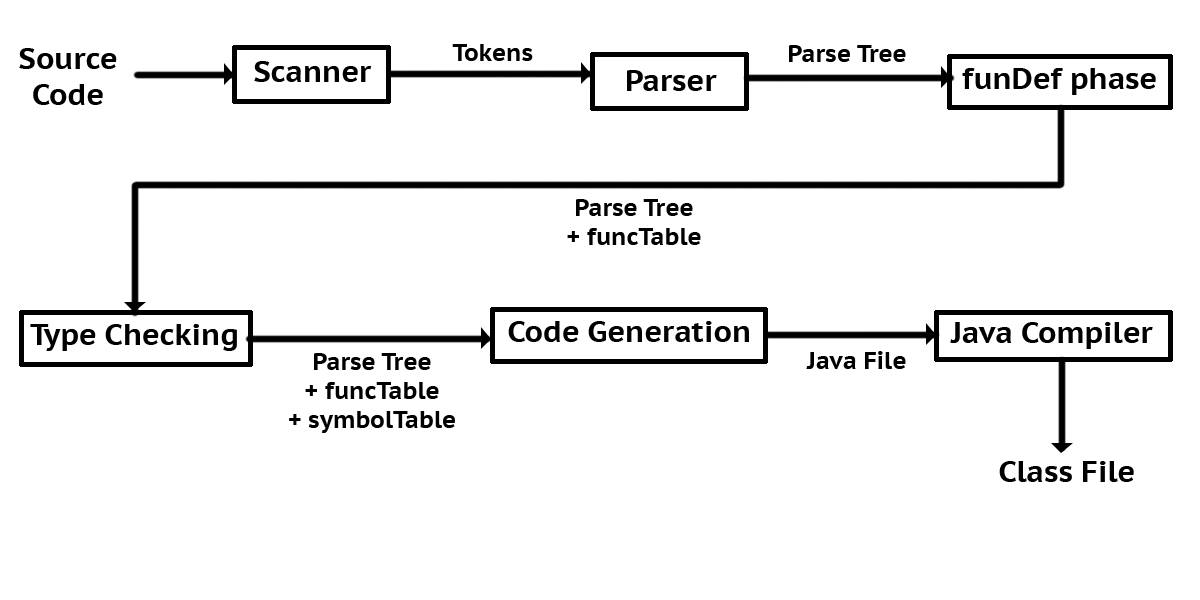
\includegraphics[scale=0.35]{billeder/compilerStructure}
\caption{Compiler structure}
\label{cs}
\end{figure}


The phases the compiler goes through are show in figure \ref{cs}. Before this though, the ANTLR tool has generated a scanner and a parser using the grammar showed in section 4.2. The ANTLR scanner is used to transform the source code into tokens. These tokens are then used by the ANTLR parser to generate the parsetree. After this the compiler does 3 triversals of this parsetree. First triversal is the funcDef phase, where every function the user has written is added to a funcTable for use in later phases. Second triversal is the Type checking phase. This phase uses a symboltable to check that the type and scope rules are followed by the code. The third triversal is the code generation phase, where the compiler goes through the parse tree and translates it to java code. Lastly the java code is sendt to the javac compiler and compiled to the finnished java robot class usable by robocode.


\section{ANTLR}
The ANTLR tool takes as input the sourcecode the user wants to parse along with the grammar for the language. It then does the lexical analysis to scan the sourcecode for compliance with the grammar to create the tokens, and after that it parses the sourcecode to create a parse tree. On top of creating the parse tree, the ANTLR tool generates 2 visitor patterns, which can be extended and used. The first and simplest is the listener. The listener has 2 functions for each node in the parse tree, one called enter and one called exit. With the listener a walker is needed to triverse the parse tree. As the walker visits nodes in the parse tree it calls the right function in the listener. The enter function is called as soon as the walker visits the node. After this the walker visits any child nodes. When it returns from these child notes the exit function is called. The second visitor pattern is the visitor. The visitor has one function per node. Each node function is responsible for calling all child node functions it has. This gives the coder more freedom in when to call the child nodes and i which order. Also the visitor supports return types on the functions, which makes it possible to pass data from one node to the caller node. 


\section{Function definition}
After ANTLR has produced the parse tree, base listener and base visitor, the function definition phase starts. In this phase every function that already exists in Robocode, will be mapped to the names defined in the appendix,(Indsæt reference til apendix her!!!!!) and added to the function table. Also every user defined function or actions will be added to this function table. 

\subsection{FuncSymbol \& FuncSymbolTable}
To keep track of the varies functions and their parameters, return values and Robocode names, a FuncSymbol class is used as representation for a single function and a FuncSymbolTable class is used to keep track of every FuncSymbol in the program.
The FuncSymbol has a string properties for Name, Type, ReturnType, original Robocode names and a string array for the parameters.

The FuncSymbolTable is basically a key/value pair HashMap. Where the key is the type of the function followed by the name of the function. The type in this case, can be either Function or Action from user defined functions, Tank, Gun, Battlefield, Radar or Utils from Robocode functions or the name of the event from Robocode events.
This class has two functions, GetFuncSymbol and EnterFuncSymbol which can be found in listing \ref{FST}. 

The GetFuncSymbol takes a type and a name from a function, combines them, looks for them in the HashMap and returns the result.

EnterFuncSymbol takes a FuncSymbol and tries to add it to the HashMap. First it checks if a function with same type and name was already declared, if such a function exists, an error is thrown, otherwise the function is added to the HashMap.

\begin{lstlisting}[caption={FuncSymbolTable}, label={FST}]
public class FuncSymbolTable {

	public LinkedHashMap<String, FuncSymbol> Map = new LinkedHashMap<String, FuncSymbol>();

	public FuncSymbol GetFuncSymbol(String type, String name){
    	FuncSymbol sym = Map.get(type + name);
    	return sym;
	}

	public void EnterFuncSymbol(FuncSymbol fs){
    	FuncSymbol oldSym = GetFuncSymbol(fs.Type, fs.Name);
    	if (oldSym != null) {
        	Error e = new Error("Function already declared");
        	throw e;
    	}
    	Map.put(fs.Type + fs.Name, fs);
	}
}
\end{lstlisting}

Forklar måden hvor på vi mapper robocode funktioner til vores funktioner
Forklar om den listener og walker vi bruger og hvordan de virker. (I hvert fald  få forklaret hvodan vi implementere dem her, hvis de er beskrevet  i den section før)
Error handling
Forklar om de to forskellige functables der bliver generete af henholdsvis bruger og fra den fil der bilver loadet ind. 

\subsection{Robocode functions \& events}
To allow the type checker and code generation phase to do their jobs, every Robocode function and event needs to be added to the FuncSymbolTable. To do this a simple text file was created which line for line have each function written out in a specific manner. 

WE COULD EXPLAIN THE TEXTFILE AND THE ALGORITHM USED TO LOAD IT IN IF WE HAVE TIME!!

\subsection{Userdefined functions \& actions}
To load the user defined functions from the program, a traverse of the parse tree is done using the ANTLR generated walker/listener. For every Function and Action the listener visits, a new FuncSymbol is created and added to the FuncSymbolTable. This is done with the FuncListener class, which extends the BaseListener ANTLR created.
 
The FuncListener class overrides the Enter/Exit Action declaration functions, the Enter/Exit Function declaration functions and the Enter parameter function. In the Enter Action and Function declaration functions, a new FuncSymbol is created called CurrentFunc. To CurrentFunc a name and a type is added, and in the Function case a return type is added as well. Name, type and return type are found using the parse tree.
In the Enter parameter function adds a new parameter to the CurrentFunc's array of parameters. 
Now in the Exit Action and Function declaration functions the CurrentFunc gets added to the FuncSymbolTable. 
The reason the CurrentFunc is added in the Exit functions, is that the walker have to visit all the parameters. 

\section{Type checking} 
After the first traversal of the parse tree using the FuncListener, every function is now defined in the function table and we can begin type checking. To do type checking a Symbol- and a SymbolTable class are used to keep track of every variable and their scope, using these two classes the SymbolTypeVisitor class checks for type compatibility. 

\subsection{Symbol \& symbol table}
Every variable in the program is represented by the Symbol class. The Symbol class has the properties String Name and Type, Symbol Var and int Depth. The Name and Type represents the name and type of the variable, the interesting parts is the Var and Depth properties. Var is a reference to a Symbol of the same name but in a higher scope, this would work as stack for all symbols of the same name, where the top of the stack will be the most inner scope and therefore the one used. The Depth property indicates the depth of the scope the symbol is in, with 0 being the global scope. 

The SymbolTable is mainly two things, the Map associates a name of a variable with a symbol as key value pairs, these symbols are the ones on top of the stack describes in the paragraph before. The scope is an array of arrays of symbols. Each index of the outer array is a scope and each inner array contains the symbols of that scope. 

The SymbolTable class has four functions: OpenScope, CloseScope, GetSymbol and EnterSymbol. 

OpenScope in listing \ref{OS} is used to open a new scope. Depth is a global variable, which keeps track of the current scope's depth. When OpenScope is run, the depth is incremented. If the Scope size is less than the depth + 1, a new array is added to the scope, otherwise the old array is cleared.

\begin{lstlisting}[caption={OpenScope function}, label={OS}]
public void OpenScope(){
    depth++;
    if (Scope.size() < depth+1){
        Scope.add(new ArrayList<Symbol>());
    }else {
        Scope.get(depth).clear();
    }
}
\end{lstlisting}

 The EnterSymbol function in listing \ref{ES}, is used to enter e new symbol into the SymbolTable. When EnterSymbol is run it firstly checks if there already exists a symbol with the same name, if this is the case it checks whether the depth of this symbol is the same depth as current scope. If the depths are the same, an error is thrown, since there can't exist two variables with the same name in the same scope. If no symbol exists in the Map or it is at another depth, a new symbol is created. This symbol gets the current depth in its depth property and it sets its var property to the old symbol. It then either replaces the new symbol with the old symbol or just adds it if the old symbol was null. 

The GetSymbol function looks up a symbol in the map and will return the name of that symbol.

\begin{lstlisting}[caption={EnterSymbol function}, label={ES}]
public void EnterSymbol(String name, String type){
    Symbol oldsym = Map.get(name);
    if (oldsym != null && oldsym.Depth == depth){
        Error e = new Error("Duplicate declaration of " + name);
        throw e;
    }else{
        Symbol newSym = new Symbol();
        newSym.Name = name;
        newSym.Type = type;
        newSym.Depth = depth;
        newSym.Var = oldsym;
        Scope.get(depth).add(newSym);
        Map.put(newSym.Name, newSym);
    }
}
\end{lstlisting}

CloseScope in listing \ref{CS}, is used to close the current scope. This is done by going through each symbol \textbf{s} at the current depth, and replacing \textbf{s} in the Map with \textbf{s.Var} which is a symbol with the same name but in a higher scope. If no such symbol exists, \textbf{s} is replaced with a null value. 

\begin{lstlisting}[caption={CloseScope function}, label={CS}]
public void CloseScope(){
    Scope.get(depth).forEach(s -> {
        Symbol prevSym = s.Var;
        Map.replace(s.Name, s, prevSym);
    });
    depth--;
}
\end{lstlisting}



\subsection{The SymbolTypeVisitor class}
The SymbolTypeVisitor class extends the BaseVisitor class from ANTLR and is the second traversal through the parse tree. It visits every single node in  the parse tree and each node return its type to the caller. At each node it is determined whether the types returned match with the expected type, errors are thrown if they don't match.

At the basic level the types are returned as they are, which is the functions visitNum, visitString and visitBool, that can be found in listing \ref{VT}.

\begin{lstlisting}[caption={SymbolTypeVisitor - visitNum, visitString and visitBool functions}, label={VT}]
@Override
public String visitNum(GrammarParser.NumContext ctx) {
    return "Num";
}

@Override
public String visitString(GrammarParser.StringContext ctx) {
    return "String";
}

@Override
public String visitBool(GrammarParser.BoolContext ctx) {
    return "Bool";
}
\end{lstlisting}

Also at the basic level variable ids are looked up in the SymbolTable and their type is returned, an error is thrown if the variable isn't found in the SymbolTable, as shown in listing \ref{VID}.

\begin{lstlisting}[caption={SymbolTypeVisitor - visitId function}, label={VID}]
@Override
public String visitId(GrammarParser.IdContext ctx) {
    String test = ctx.getText();
    Symbol sym = ST.GetSymbol(ctx.getText());
    if (sym == null){
        Error e = new Error("Error at line: " +
                ctx.start.getLine() + ": Variable not found");
        throw e;
    }
    return sym.Type;
}
\end{lstlisting}

When visiting and, or, minus, not, mul, rel and eq expressions each expression type is calculated and compared to what is expected. Afterwards either an error is thrown or the right type is returned. An example of such function is the or-expression, which can be found in listing \ref{VOR}.

\begin{lstlisting}[caption={SymbolTypeVisitor - visitOrexpr function}, label={VOR}]
@Override
public String visitOrexpr(GrammarParser.OrexprContext ctx) {
    String left = visit(ctx.expr(0));
    String right = visit(ctx.expr(1));
    if (left.equals("Bool") && right.equals("Bool")){
        return "Bool";
    }else{
        Error e = new Error("Error at line: " +
                ctx.start.getLine() + ": Expression did not evaluate to Bool.");
        throw e;
    }
}
\end{lstlisting}

The add-expression in listing \ref{VADD}, is a bit special as the plus operator can be used on two numbers or a string and any other type. Therefore the function checks if both expressions evaluate to a number, or one of them is a string and the operator is a plus, it throws an error if none of the above is true else it returns the appropriate type. 

\begin{lstlisting}[caption={SymbolTypeVisitor - visitAddexpr function}, label={VADD}]
@Override
public String visitAddexpr(GrammarParser.AddexprContext ctx) {
    String left = visit(ctx.expr(0));
    String right = visit(ctx.expr(1));
    if (left.equals("Num") && right.equals("Num")) {
        return "Num";
    }else if((left.equals("String") || right.equals("String")) && ctx.op.getText().equals("+") ) {
        return "String";
    }else{
        Error e = new Error("Error at line: " +
                ctx.start.getLine() + ": Expression types did not match.");
        throw e;
    }
}
\end{lstlisting}

The function visitAssign in listing \ref{VAS}, checks whether the type of the symbol found from the id = the expression's type. It throws errors if the id doesn't match any symbols or the types don't match. 

\begin{lstlisting}[caption={SymbolTypeVisitor - visitAssign function}, label={VAS}]
@Override
public String visitAssign(GrammarParser.AssignContext ctx) {
    String id = ctx.ID().getText();
    Symbol sym = ST.GetSymbol(id);
    if (sym == null){
        Error e = new Error("variable not found");
        throw e;
    }
    if (!sym.Type.equals(visit(ctx.expr()))){
        Error e = new Error("Error at line: " +
                ctx.expr().start.getLine() + ": Expression and variable are not type compatible");
        throw e;
    }
    return sym.Type;
}
\end{lstlisting}

The function visitVardcl in listing \ref{VAD}, enters a new symbol in the SymbolTable. The type is found at the variable declaration Node or at the assign node. visitVardcl determines where to find the id and adds the new symbol to the SymbolTable. 

\begin{lstlisting}[caption={SymbolTypeVisitor - visitVardcl function}, label={VAD}]
@Override
public String visitVardcl(GrammarParser.VardclContext ctx) {
    if (ctx.getChild(1) instanceof GrammarParser.AssignContext){
        ST.EnterSymbol(((GrammarParser.AssignContext) ctx.getChild(1)).ID().getText(), ctx.TYPE().getText());
        visit(ctx.assign());
    }else {
        ST.EnterSymbol(ctx.ID().getText(), ctx.TYPE().getText());
    }
    return ctx.TYPE().getText();
}
\end{lstlisting}

The visitBlock function in listing \ref{VB}, opens a new scope and if its parent is the Action declaration, any parameter of the Action declaration  is added to the scope. The function then visits all the statements in the block and then closes the scope. 

\begin{lstlisting}[caption={SymbolTypeVisitor - visitBlock function}, label={VB}]
@Override
public String visitBlock(GrammarParser.BlockContext ctx) {
    ST.OpenScope();
    if (ctx.parent instanceof GrammarParser.ActdclContext){
        FuncSymbol fs = FST.GetFuncSymbol("Action", ((GrammarParser.ActdclContext) ctx.parent).ID().getText());
        fs.Params.forEach(tuple -> {
            ST.EnterSymbol(tuple.x, tuple.y);
        });
    }
    visit(ctx.stmts());
    ST.CloseScope();
    return "null";
}
\end{lstlisting}

The function visitArgs in listing \ref{VAF} at line 1-8, visits each expression and concatenates with a comma in between and returns the whole thing as a string. 

visitFcall which is also found in listing \ref{VAF} at line 10-37, gets a function symbol from the FuncSymbolTable and then matches each argument type from the visitArgs with each parameter type in the function symbol. Errors are thrown if these don't match or the function id doesn't match any function in the FuncSymbolTable. visitAcall, visitUtilscall, visitBattlefieldcall, visitRadarcall, visitGuncall and visitTankcall functions works similarly to the visitFcall function.

\begin{lstlisting}[caption={SymbolTypeVisitor - visitArgs and visitFcall functions}, label={VAF}]
@Override
public String visitArgs(GrammarParser.ArgsContext ctx) {
    String result = visit(ctx.expr(0));
    for (int i = 1; i < ctx.expr().size(); i++){
        result = result + ", " + visit(ctx.expr(i));
    }
    return result;
}

@Override
public String visitFcall(GrammarParser.FcallContext ctx) {
    FuncSymbol fsym = FST.GetFuncSymbol("Function", ctx.ID().getText());
    if (fsym == null){
        Error e = new Error("Error at line: " +
                ctx.start.getLine() + ": Function not found");
        throw e;
    }
    if (!fsym.Type.equals("Function")){
        Error e = new Error("Error at line: " +
                ctx.start.getLine() + ": Incorrect function type.");
        throw e;
    }
    if(ctx.getChildCount() == 4) {
        String[] args = visit(ctx.args()).split(", ");
        for (int i = 0; i < args.length; i++) {
            String paramType = fsym.Params.get(i).y;
            String arg = args[i];
            if (!paramType.equals(arg)) {
                Error e = new Error("Error at line: " +
                        ctx.args().expr(i).start.getLine() +
                        ": Parameter number " + i + " not matched. Expected " + paramType);
                throw e;
            }
        }
    }
    return fsym.ReturnType;
}
\end{lstlisting}

visitEcall in listing \ref{VE}, is a bit special compared to the other call function, as it needs to check whether the function called is comparable with the event that it is called within. To do this, it checks the parent to see if that is an event declaration, if it is not, it checks the parent of the parent and so on, until it either reaches the event declaration or the root of the tree, if the root is reached an error is then thrown. If an event declaration is reached, the event declaration id and the event call id is used to look up the function in the FuncSymbolTable, if none is returned an error is thrown, otherwise the arguments are matched with the parameters as before, if successful the function's return type is returned. 

\begin{lstlisting}[caption={SymbolTypeVisitor - visitEcall function}, label={VE}]
@Override
public String visitEcall(GrammarParser.EcallContext ctx) {
    RuleContext parent = ctx.parent;
    while(parent != null){
        if(parent instanceof GrammarParser.EventdclContext){
            FuncSymbol fsym = RoboFST.GetFuncSymbol(((GrammarParser.EventdclContext) parent).ID().getText(), ctx.ID().getText());
            if (fsym == null){
                Error e = new Error("Error at line: " +
                        ctx.start.getLine() + ": Function not found");
                throw e;
            }
            if(ctx.getChildCount() == 5) {
                String[] args = visit(ctx.args()).split(", ");
                for (int i = 0; i < args.length; i++) {
                    String paramType = fsym.Params.get(i).y;
                    String arg = args[i];
                    if (!paramType.equals(arg)) {
                        Error e = new Error("Error at line: " +
                                ctx.args().expr(i).start.getLine() +
                                ": Parameter number " + i + " not matched. Expected " + paramType);
                        throw e;
                    }
                }
            }
            return fsym.ReturnType;
        }
        parent = parent.parent;
    }
    Error e = new Error("Event calls must be inside an event/when function");
    throw e;
}
\end{lstlisting}

visitDcls makes sure that the program the user wrote has one and only one Tankname, Repeatblock and Setupblock declared. 

\begin{lstlisting}[caption={SymbolTypeVisitor - visitDcls function}, label={VD}]
@Override
public String visitDcls(GrammarParser.DclsContext ctx) {
    if (ctx.tankname().size() < 1){
        Error e = new Error("A Tankname needs to be declared");
        throw e;
    }else if (ctx.tankname().size() > 1){
        Error e = new Error("Error at line: " +
                ctx.tankname(1).start.getLine() + ": Too many tank names.");
        throw e;
    }
    if (ctx.repeatblock().size() < 1){
        Error e = new Error("A Repeat block needs to be declared");
        throw e;
    }else if (ctx.repeatblock().size() > 1){
        Error e = new Error("Error at line: " +
                ctx.repeatblock(1).start.getLine() + ": Too many repeat blocks.");
        throw e;
    }
    if (ctx.setupblock().size() < 1){
        Error e = new Error("A Setup block needs to be declared");
        throw e;
    }else if (ctx.setupblock().size() > 1){
        Error e = new Error("Error at line: " +
                ctx.setupblock(1).start.getLine() + ": Too many setup blocks.");
        throw e;
    }
    super.visitDcls(ctx);
    return "null";
}
\end{lstlisting}



Forklar vi "overskriver" visitoren, eller vi bruger visitoren.
\section{Code generation}
The CodeGen class extends the BaseListener class and is the third and last traversal of the parse tree. At this point the program is type checked and ready to get translated into Java code, the CodeGen class generates a string containing the translated code. 

When visiting the literals bool, num and string nothing is changed and the text is returned. When visiting id an "\_" is added in front of the id, to make sure the id name doesn't clash with Java keywords. The literals id and num can be seen in listing \ref{VIM}. 

\begin{lstlisting}[caption={CodeGen - visitId \& visitNum functions}, label={VIM}]
@Override
public String visitId(GrammarParser.IdContext ctx) {
    return "_" + ctx.ID().getText();
}

@Override
public String visitNum(GrammarParser.NumContext ctx) {
    return ctx.NUM().getText();
}
\end{lstlisting}

When visiting expressions the only thing needed is to change AND, OR, IS=, NOT= and NOT is changed to their equivalent operator in Java. 

In the visitEcall function in listing \ref{VEC} the appropriate FuncSymbol is found in the FuncSymbolTable using the same method as the SymbolTypeVisitor class. visitEcall adds "e." in front of the function name, before it returns. The "e" will be the parameter of the event which this call is within. 

\begin{lstlisting}[caption={CodeGen - visitEcall function}, label={VEC}]
@Override
public String visitEcall(GrammarParser.EcallContext ctx) {
    FuncSymbol fsym;
    RuleContext parent = ctx.parent;
    while(parent != null){
        if(parent instanceof GrammarParser.EventdclContext){
            fsym = RoboFST.GetFuncSymbol(((GrammarParser.EventdclContext) parent).ID().getText(), ctx.ID().getText());
            if(ctx.getChildCount() == 5) {
                return "e." + fsym.RoboCodeName + "(" + visit(ctx.args()) + ")";
            }else {
                return "e." + fsym.RoboCodeName + "()";
            }
        }
        parent = parent.parent;
    }
    Error e = new Error("codeGen Error");
    throw e;
}
\end{lstlisting}

In all other Robocode calls, like the visitTankcall function found in listing \ref{VTC}, the appropriate FuncSymbol is found in the FuncSymbolTable and the Robocode name is returned with potential arguments.

\begin{lstlisting}[caption={CodeGen - visitTankcall function}, label={VTC}]
@Override
public String visitTankcall(GrammarParser.TankcallContext ctx) {
    FuncSymbol fs = RoboFST.GetFuncSymbol("Tank", ctx.ID().getText());
    if(ctx.getChildCount() == 5) {
        return fs.RoboCodeName + "(" + visit(ctx.args()) + ")";
    }else {
        return fs.RoboCodeName + "()";
    }
}
\end{lstlisting}

In Function and Action calls an "\_" are added in front of the id and potential parameters before returning. This is done like with the num, string and bool literals, so the id's don't clash with any Java keywords. Listing \ref{VFC} shows the visitFcall function.

\begin{lstlisting}[caption={CodeGen - visitFcall function}, label={VFC}]
@Override
public String visitFcall(GrammarParser.FcallContext ctx) {
    if (ctx.getChildCount() == 4){
        return "_" + ctx.ID().getText() + "(" + visit(ctx.args()) + ")";
    }else{
        return "_" + ctx.ID().getText() + "()";
    }
}
\end{lstlisting}

The visitIfstmt function uses a StringBuilder to add the \textbf{if} followed by any \textbf{elseif} if needed, at the end the StringBuilder returns as a string. The visitIfstmt function is shown in listing \ref{VISTM}

\begin{lstlisting}[caption={CodeGen - visitIfstmt function}, label={VISTM}]
@Override
public String visitIfstmt(GrammarParser.IfstmtContext ctx) {
    StringBuilder buf = new StringBuilder();
    buf.append("if(");
    buf.append(visit(ctx.expr()));
    buf.append(")");
    buf.append(visit(ctx.block(0)));
    for(int i = 0; i< ctx.elseif().size(); i++){
        buf.append(visit(ctx.elseif(i)));
    }
    if (ctx.block().size() > 1){
        buf.append("else");
        buf.append(visit(ctx.block(1)));
    }
    return buf.toString();
}
\end{lstlisting}

The visitVardcl function shown in listing \ref{VVDCL}, changes the type declared in the program to the equivalent type in Java. String and Bool will be changes to string and boolen, where the type Num will be changed to a double. Another thing worth mentioning is the "\_" in front of the ids, for the same reasons as mentioned before.

\begin{lstlisting}[caption={CodeGen - visitVardcl function}, label={VVDCL}]
@Override
public String visitVardcl(GrammarParser.VardclContext ctx) {
    String result;
    if (ctx.TYPE().getText().equals("Num")){
        result = "double ";
    }else if(ctx.TYPE().getText().equals("Bool")){
        result = "boolean ";
    }else{
        result = "String ";
    }
    if (ctx.getChild(1) instanceof GrammarParser.AssignContext){
        result += visit(ctx.assign());
    }else {
        result += "_" + ctx.ID().getText() + ctx.SEMI().getText() + "\n";
    }
    return result;
}
\end{lstlisting}

The visitEventdcl function in listing \ref{VEDCL} is worth noting the added "on"  and the added "Event", these are used to create the Robocode eventhandler and the Robocode event. The "e" added after "Event" corresponds to the e in visitEcall.

\begin{lstlisting}[caption={CodeGen - visitEventdcl function}, label={VEDCL}]
@Override
public String visitEventdcl(GrammarParser.EventdclContext ctx) {
    String id = StringUtils.capitalize(ctx.ID().getText());
    return "public void on" + id + "( " + id + "Event e )" + visit(ctx.block());
}
\end{lstlisting}

In the visitFuncdcl function  a new public Java function is created with the return type with the appropriate return type, name, block and possibly parameters. Once again an "\_" is added in front of the id, for the same reasons as before.

\begin{lstlisting}[caption={CodeGen - visitFuncdcl function}, label={VFDCL}]
@Override
public String visitFuncdcl(GrammarParser.FuncdclContext ctx) {
    String type;
    if (ctx.TYPE().getText().equals("Num")){
        type = "double ";
    }else if(ctx.TYPE().getText().equals("Bool")){
        type = "boolean ";
    }else{
        type = "String ";
    }
    if (ctx.getChildCount() == 8) {
        return "public " + type + " _" + ctx.ID().getText() + "(" + visit(ctx.params()) + ")" + visit(ctx.functionBlock());
    }else{
        return "public " + type + " _" + ctx.ID().getText() + "()" + visit(ctx.functionBlock());
    }
}
\end{lstlisting}

The visitSetupblock and visitRepeatblock functions shown in listing \ref{VSRB} are a bit special as the Repeat block(is the while(true) statement in the Run function in Java) is inside the Setup block(Run function) in Java. To do this Setup block creates the void function and adds the block, then cuts of the last curly bracket adds the Repeat block, which is renamed to while(true) and puts back the curly bracket. 

\begin{lstlisting}[caption={CodeGen - visitSetupblock \& visitRepeatblock functions}, label={VSRB}]
@Override
public String visitSetupblock(GrammarParser.SetupblockContext ctx) {
    String result = "public void run()" + visit(ctx.block());
    result = result.substring(0, result.length()-2);
    return result + visit(((GrammarParser.DclsContext) ctx.parent).repeatblock(0)) + "}";
}

@Override
public String visitRepeatblock(GrammarParser.RepeatblockContext ctx) {
    return "while (true)" + visit(ctx.block());
}
\end{lstlisting}

In the visitProg function a StringBuilder is used to add the import statements needed for Java to be able to compile the program. After that the class is declared using the Tankname and then extends Robot to the class declaration. After this the entire program is added followed by a closing curly bracket. The code generation is now complete and a string with the entire program in Java code is returned. 

\begin{lstlisting}[caption={CodeGen - visitProg function}, label={VP}]
@Override
public String visitProg(GrammarParser.ProgContext ctx) {
    StringBuilder buf = new StringBuilder();
    buf.append("import robocode.*;\n");
    buf.append("import static robocode.util.Utils.*;\n");
    buf.append("public class ");
    buf.append(StringUtils.capitalize(visit(ctx.dcls().tankname(0))));
    buf.append(" extends Robot {\n ");
    buf.append(visit(ctx.dcls()));
    buf.append("}");
    System.out.print(buf.toString());
    return buf.toString();
}
\end{lstlisting}


TO DO
Rename Txt og TEXT til String.
Open og close scope i functionBlockContext
CodeGen errors
Ændre while i codegen
Lav billede til Environment store model, og forklar det!
Apendix, skriv tekst til det vi har, overvej om der skal tilføjes kode eksempler.
Formuler en problem stilling i introduction.



\chapter{Tests}
This chapter is covering the tests that has been done to confirm the functionality of our language. Two kinds of tests will be used, convertion tests where the language will be used in practice and unit tests with focus on making sure everything works as planned.


\section{Convertion tests}
In this section tests will be run where sample robots from Robocode will be written in our language, compiled back to Java and compared with the original robot. The focus of this test is to make sure that the language works in practice. Doing work and documenting any errors found while using the language quickly helped discovering some problems which then could be fixed. 

\subsection{Tracker}
When writing the robot Tracker in our language a few errors were found. First an error was received that the Expression types didn't match for an assignment. This was quickly fixed as it turned out the Utils.normalRelativeAngleDegrees had the wrong returntype in the ReservedFunctions list.

Another error occurred were the compiler returned the error Variable not found. This was fixed by changning trackName = null to trackName = "0" throughout the code when a target has not been found. The compiler also gives an error if a robot has been given another name in the code than in the file name.

To test if the converted version of Tracker works the same as the original version both robots has been tested versus the sample robot Crazy. The output log of Robocode shows that the converted version has a problem with an if-statement checking whether the robot it hits is the same as the target. Looking at the scoreboard of the match the converted robot earns 20\% less points than the original sample robot. This shows that there has been a flaw in the conversion and that the robots does not share the exact same functionality.
There are two main causes for this problem. The first cause is that the Robocode command \emph{setAdjustGunForRobotTurn(true)} is not implemented in our language. The second cause is that it's not possible to use a return statement inside an if-statement in our language.


\subsection{Fire}
When converting the Fire robot to our language there was an error in the compiler saying that the variable was not found. This error occurred because the variable Num dist was declared in the setup block, it was fixed by moving the declaration outside the block.

When testing the converted Fire robot versus the sample Fire robot by matching both robots against the Crazy sample robot, both versions of the Fire robot behaved in the same way and earned scores close to each other.
This shows that the robot has been compiled to have the same functionality after being written in our language as the original sample robot.




%% Teknisk %%


%% Afrunding %%
\chapter{Discussion}
\label{chap:Discussion}

Error handling - evt. med en error stack ?
Vi kunne have haft ét symbol table?
Tjekke efter moscow,
Generelt hvad vi har opnået


In section \ref{sec:MoSCoW} the MoSCoW analysis was created and described. The method was used to prioritize the requirements for the project's language. Table \ref{moscowDis} shows which of the requirements that have been implemented and which have not been implemented. \newline
All \textit{Must have} requirements has been implemented as they should, since these were the most important and essential requirements for the language. These were needed to make the logic, movement etc., for the robot. \newline
All \textit{Should have} requirements has also been implemented. The Events and Void and type methods helps the users in order to make more intelligent robots, where Comments are useful for the readability of the program, made by the user. \newline
Most of the requirements in \textit{Could have}, has been implemented, which is Print statements, Strings and Setup block. Print statements and Strings have been implemented for the user to be able to debug their code. The Setup block is used for code, that should only be run once each round. Here the user could write code to make some initializing movements e.g. make the  robot move to the wall. Cos, Sin \& Tan and For loops were not implemented in DatLanguage. \newline
None of the requirements from \textit{Won't have} were implemented in this project.

\begin{table}[H]
\centering
\begin{tabular}{ |l|l|l| }
\hline
\multicolumn{3}{ |c| }{MoSCoW analysis} \\
\hline
& MoSCoW items & Status \\
\hline
\multirow{7}{*}{Must have} & Primitive types and variables & Implemented \\
& While loop & Implemented \\
& Reserved calls & Implemented \\
& Robot naming & Implemented \\
& If/Else/Elseif statements & Implemented \\
& Arithmetic expressions and operators & Implemented \\
& Logical expressions and operators & Implemented \\ \hline
\multirow{3}{*}{Should have} & Events & Implemented \\
& Comments & Implemented \\
& Void and type methods & Implemented \\ \hline
\multirow{6}{*}{Could have} & Cos, Sin \& Tan & {\color{red}Not Implemented} \\
& For loops & {\color{red}Not Implemented} \\
& Print statements & Implemented \\
& Strings & Implemented \\
& Setup block & Implemented  \\ \hline
\multirow{3}{*}{Won't have} & Random number generator & {\color{red}Not Implemented} \\
& Other robot types & {\color{red}Not Implemented} \\
\hline
\end{tabular}
\caption{Fulfilment of the MoSCoW analysis}
\label{moscowDis}

\end{table}
\chapter{Conclusion}


\include{formalia/futurework}

%%%% Kilder %%%%

\begingroup
	\raggedright
	\bibliography{bibtex/litteratur}							% Litteraturlisten inkluderes
\endgroup


%%%% Fixme-listen %%%%

\newpage														% Ny side til Fixme-listen
%\listoffixmes													% Fixme-listen - fjernes til sidst i projektet med "%"


%%%% Appendiks %%%%

\appendix														% Appendiks/bilag start - giver chapter bogstaver i stedet for tal
\clearforchapter												% Sikrer at pagestylen aktiveres paa den rigtige side
\phantomsection													% Kunstigt afsnit, som hyperlinks kan 'holde fast i'
\pdfbookmark[0]{Appendiks}{appendiks}							% Tildeler en klikbar bookmark til den endelige PDF

%% Indstillinger for appendiks (deaktiveret med "%") %%

%\pagestyle{empty}												% Sidehoved/-fod for standardsider aendres til tom for appendiks
%\aliaspagestyle{chapter}{empty}								% Sidehoved/-fod for kapitelsider aendres til tom for appendiks
%\settocdepth{chapter}											% Kun kapitel-niveau vises i ToC
%\addtocontents{toc}{\protect\cftpagenumbersoff{chapter}}		% Sidetal for kapitler fjernes i ToC

%% Filer til appendiks %%

\chapter{Appendiks name} \label{sec:ap1}
\begin{center}
    \begin{tabular}{ | l| l | p{0.5\linewidth} | }
    \hline
    Reserved calls & Our language & RoboCode \\ \hline
    Tank. & forward(num distance) & ahead(double distance)  \\ \hline
     & backward(num distance) & back(double distance)  \\ \hline
     & doNothing() & doNothing() \\ \hline
     & energy() & getEnergy() \\ \hline
     & heading() & getHeading() \\ \hline
     & height() & getHeight() \\ \hline
     & width() & getWidth()  \\ \hline
     & velocity() & getVelocity()  \\ \hline
     & xCoord() & getX() \\ \hline
     & yCoord & getY() \\ \hline
     & stop() & stop() \\ \hline
     & resume() & resume() \\ \hline
     & turn(num degrees) & turnLeft(double degrees)  \\ \hline
     & &  \\ \hline
    Gun. & shoot(num power) & fire(double power) \\ \hline
     & coolingRate() & getGunCoolingRate() \\ \hline
     & heading() & getGunHeading() \\ \hline
     & heat() & getGunHeat() \\ \hline
     & turn(num ddegrees) & turnGunLeft(double degrees)  \\ \hline
     & adjustGunForRobotTurn(boolean) & adjustGunForRobotTurn(boolean independant) \\ \hline
     & &  \\ \hline
    Radar. & heading() & getRadarHeading() \\ \hline
     & scan() & scan() \\ \hline
     & adjustRadarForGunTurn(boolean) & adjustRadarForGunTurn(boolean independant)  \\ \hline
     & adjustRadarForRobotTurn(boolean) & adjustRadarForRobotTurn(boolean independant) \\ \hline
     & turn(num degrees) & turnRadarLeft(double degrees) \\ \hline
     & &  \\ \hline
    Battlefield. & height() & getBattleFieldHeight() \\ \hline
     & width() & getBattleFieldWidth() \\ \hline
     & numOfRounds() & getNumRounds() \\ \hline
     & enemies() & getOthers() \\ \hline
     & roundNum() & getRoundNum() \\ \hline
     & time() & getTime()  \\
    \hline
    \end{tabular}
\end{center}

\begin{center}
	\begin{tabular}{ | p{0.3\linewidth} | p{0.3\linewidth} | p{0.3\linewidth} |}
		\hline
		OL / Robocode Event& OL Event Information & Robocode Event Information \\ \hline
		BulletHit / onBulletHit& bulletHeading() & getBullet().getHeading() \\ \hline
		& bulletOwner() & getBullet().getName() \\ \hline
		& bulletPower() & getBullet().getPower() \\ \hline
		& bulletVelocity() & getBullet().getVelocity() \\ \hline
		& bulletVictim() & getBullet().getVictim() \\ \hline
		& bulletXCoord() & getBullet().getX() \\ \hline
		& bulletYCoord() & getBullet().getY() \\ \hline
		& bulletIsActive() & getBullet().isActive() \\ \hline
		& energy() & getEnergy() \\ \hline
		BulletHitBullet / onBulletHitBullet& bulletHeading() & getBullet().getHeading() \\ \hline
		& bulletOwner() & getBullet().getName() \\ \hline
		& bulletPower() & getBullet().getPower() \\ \hline
		& bulletVelocity() & getBullet().getVelocity() \\ \hline
		& bulletVictim() & getBullet().getVictim() \\ \hline
		& bulletXCoord() & getBullet().getX() \\ \hline
		& bulletYCoord() & getBullet().getY() \\ \hline
		& bulletIsActive() & getBullet().isActive() \\ \hline
		& enemyBulletHeading() & getHitBullet().getHeading() \\ \hline
		& enemyBulletOwner() & getHitBullet().getName() \\ \hline
		& enemyBulletPower() & getHitBullet().getPower() \\ \hline
		& enemyBulletVelocity() & getHitBullet().getVelocity() \\ \hline
		& enemyBulletVictim() & getHitBullet().getVictim() \\ \hline
		& enemyBulletXCoord() & getHitBullet().getX() \\ \hline
		& enemyBulletYCoord() & getHitBullet().getY() \\ \hline
		& enemyBulletIsActive() & getHitBullet().isActive() \\ \hline
		HitByBullet / onHitByBullet& bearing() & getBearing() \\ \hline
		& bearingDegrees() & getBearingDegrees \\ \hline
		& bulletHeading() & getBullet().getHeading() \\ \hline
		& bulletOwner() & getBullet().getName() \\ \hline
		& bulletPower() & getBullet().getPower() \\ \hline
		& bulletVelocity() & getBullet().getVelocity() \\ \hline
		& bulletVictim() & getBullet().getVictim() \\ \hline
		& bulletXCoord() & getBullet().getX() \\ \hline
		& bulletYCoord() & getBullet().getY() \\ \hline
		& bulletIsActive() & getBullet().isActive() \\ \hline
		& heading() & getHeading() \\ \hline
		& headingDegrees() & getHeadingDegrees() \\ \hline
		& power() & getPower() \\ \hline
		& velocity() & getVelocity() \\ \hline
		HitRobot / onHitRobot & bearing() & getBearing() \\ \hline
		& bearingDegrees() & getBearingDegrees \\ \hline
		& energy() & getEnergy() \\ \hline
		& myFault() & isMyFault() \\ \hline
		& enemyName() & getName() \\ \hline
		Death / onDeath & & \\ \hline
		HitWall / onHitWall & bearing() & getBearing() \\ \hline
		EnemyDeath / onRobotDeath & enemyName() & getName() \\ \hline
		RoundEnded / onRoundEnded & round() & getRound() \\ \hline
		& totalTurns() & getTotalTurns() \\ \hline
		& turns() & getTurns() \\ \hline
		ScannedRobot / onScannedRobot & bearing() & getBearing() \\ \hline
		& distance() & getDistance() \\ \hline
		& energy() & getEnergy() \\ \hline
		& heading() & getHeading() \\ \hline
		& enemyName() & getName() \\ \hline
		& velocity() & getVelocity() \\ \hline
		Status / onStatus & distanceRemaining() & getStatus.getDistanceRemaining() \\ \hline
		& gunTurnRemaining() & getStatus.getGunTurnRemaining() \\ \hline
		& radarTurnRemaining() & getStatus.getRadarTurnRemaining() \\ \hline
		Win / onWin &  & \\
		\hline
	\end{tabular}
\end{center}


%%%% Bilag %%%%

%\phantomsection												% Kunstigt afsnit, som hyperlinks kan 'holde fast i'
%\addcontentsline{toc}{chapter}{Bilag A \ Navn} 				% Manuelle indgange i indholdsfortegnelsen (naar \includepdf bruges)

%\includepdf[pages={x-y}]{filnavn}								% Inkluder eksterne bilag med \includepdf[pages={x-y}]{filnavn}


\end{document}													% Slutter dokumentet - obligatorisk


